% Гайд «Геометрія токамака: від ψ(R,Z) до котушок JET»
% Компіляція: latexmk main.tex   (latexmkrc вмикає XeLaTeX, -shell-escape і Pygments для minted)
% Числа й рисунки: code/geom_tour.py (див. розд. 1).
\documentclass[11pt,a4paper,oneside,notitlepage]{report}
% Преамбула гайду по геометрії: копія guide/preamble.tex (ті самі рамки, \code, notation.sty)
% + шлях до рисунків методички + рамки «Модель проєкту» і «Нове спостереження».

% ---------- мова і шрифти ----------
\usepackage{fontspec}
\usepackage{polyglossia}
\setdefaultlanguage{ukrainian}
\setotherlanguage{english}
\gappto\captionsukrainian{\renewcommand{\bibname}{Бібліографія}\renewcommand{\refname}{Бібліографія}}
\setmainfont{cmunrm}[Extension=.otf,BoldFont=cmunbx,ItalicFont=cmunti,BoldItalicFont=cmunbi]
\setsansfont{cmunss}[Extension=.otf,BoldFont=cmunsx,ItalicFont=cmunsi,BoldItalicFont=cmunso]
\setmonofont{cmuntt}[Extension=.otf,BoldFont=cmuntb,ItalicFont=cmunit,BoldItalicFont=cmuntx]

% ---------- верстка ----------
\usepackage[a4paper,top=2cm,bottom=2.2cm,left=2.2cm,right=2cm]{geometry}
\usepackage{titlesec}
\titleformat{\chapter}[hang]{\Large\bfseries\sffamily}{\thechapter.}{0.6em}{}
\titlespacing*{\chapter}{0pt}{-10pt}{12pt}
\titleformat{\section}{\large\bfseries\sffamily}{\thesection}{0.6em}{}
\titleformat{\subsection}{\normalsize\bfseries\sffamily}{\thesubsection}{0.6em}{}
\usepackage{enumitem}
\usepackage{tocloft}
\usepackage{multicol}
\setlength{\cftbeforechapskip}{2pt}
\renewcommand{\cftsecfont}{\small}\renewcommand{\cftsecpagefont}{\small}
\setlength{\cftbeforetoctitleskip}{0pt}
\renewcommand{\cfttoctitlefont}{\large\bfseries\sffamily}
\setlength{\cftaftertoctitleskip}{4pt}
\setlength{\cftbeforesecskip}{0pt}

\setlist{itemsep=1pt,topsep=3pt,parsep=0pt}
\setlength{\emergencystretch}{3em}% довгі шляхи файлів у \texttt
\usepackage{booktabs,array,tabularx,longtable}
\renewcommand{\arraystretch}{1.12}
\usepackage{graphicx}
\graphicspath{{figures/}{../manual/figures/}}
\usepackage[font=small,labelfont=bf,labelsep=period]{caption}
\usepackage{subcaption}
\usepackage[table]{xcolor}
\usepackage{tikz}
\usetikzlibrary{arrows.meta,calc,decorations.markings,positioning,shapes.geometric}

% ---------- математика і позначення ----------
\usepackage{notation}
\numberwithin{equation}{chapter}

% ---------- рамки ----------
\usepackage[most]{tcolorbox}
\tcbset{enhanced,breakable,boxrule=0.5pt,arc=1.5pt,left=5pt,right=5pt,top=3pt,bottom=3pt,
        fonttitle=\sffamily\bfseries\small\hypersetup{citecolor=white,linkcolor=white},before skip=6pt,after skip=6pt}
% стандартна теорія поза корпусом (рішення Q1)
\newtcolorbox{outofcorpus}[1][]{colback=gray!5,colframe=gray!60!black,
  title={Поза корпусом: стандартна теорія\ifx&#1&\else{} --- #1\fi}}
% приклад з корпусу: реальні установки й числа
\newtcolorbox{corpusexample}[1][]{colback=blue!3,colframe=blue!50!black,
  title={Приклад з корпусу\ifx&#1&\else{} --- #1\fi}}
% виведення з пропущеними рутинними кроками
\newtcolorbox{derivation}[1][]{colback=white,colframe=black!40,
  title={Виведення\ifx&#1&\else{} --- #1\fi}}
% практикум на коді проєкту
\newtcolorbox{practicum}[1][]{colback=green!4,colframe=green!40!black,
  title={Практикум\ifx&#1&\else{} --- #1\fi}}
% дослідницький трек: статуси з реєстрів Our try/00-decisions
\newtcolorbox{established}[1]{colback=teal!4,colframe=teal!60!black,
  title={Встановлено в проєкті [#1]}}
\newtcolorbox{conjecture}[1]{colback=orange!6,colframe=orange!70!black,
  title={Гіпотеза [#1] --- не перевірено}}
\newtcolorbox{refuted}[1]{colback=red!4,colframe=red!55!black,
  title={Спростовано [#1] --- повчальний приклад}}


% ---------- код (путівник) ----------
% minted (Pygments через latexminted); збірка: latexmk (див. latexmkrc: -shell-escape, PATH до Pygments).
% listings відмовились: під XeLaTeX він зсуває нумерацію, якщо над фрагментом є не-ASCII символи.
\usepackage{minted}
\usepackage{needspace}
\setminted{fontsize=\scriptsize,linenos,numbersep=6pt,breaklines,breakanywhere,frame=single,
  framesep=2mm,rulecolor=black!25,bgcolor=black!2,style=default}
% \code{шлях}{перший}{останній}{підпис} — фрагмент БЕЗПОСЕРЕДНЬО з файлу проєкту (через src/-посилання)
\newcommand{\code}[4]{\par\needspace{7\baselineskip}\noindent
  {\footnotesize\texttt{\detokenize{#1}}, рядки #2--#3\quad #4}\par\nopagebreak[4]\vspace{-2pt}
  \inputminted[firstline=#2,lastline=#3,firstnumber=#2]{python}{src/#1}}
% ---------- рамки гайду ----------
\newtcolorbox{projmodel}[1][]{colback=violet!4,colframe=violet!55!black,
  title={Модель проєкту\ifx&#1&\else{} --- #1\fi}}
\newtcolorbox{newfinding}[1][]{colback=yellow!7,colframe=yellow!45!black,
  title={Нове спостереження (не внесено в реєстри)\ifx&#1&\else{} --- #1\fi}}
\newtcolorbox{cheat}[1][]{colback=black!2,colframe=black!45,
  title={Шпаргалка\ifx&#1&\else{} --- #1\fi}}
% ---------- картки пунктів реєстру ----------
\newtcolorbox{itemcard}[2]{colback=black!2,colframe=black!55,title={#1\quad\normalfont\small #2}}

% ---------- посилання ----------
\usepackage[colorlinks=true,linkcolor=blue!50!black,citecolor=green!40!black,
            urlcolor=blue!60!black,bookmarksnumbered]{hyperref}
\usepackage{xurl}
\usepackage[ukrainian,nameinlink]{cleveref}

\title{Геометрія токамака: гайд}
\author{Проєкт «Моделювання потоку плазми в контурі токамаку»}
\date{2026}

\begin{document}
\thispagestyle{plain}
\begin{center}
{\LARGE\bfseries\sffamily Геометрія токамака}\\[3pt]
{\large\sffamily Гайд: координати, магнітні поверхні, форма перерізу, топологія і JET --- з кодом проєкту}\\[2pt]
{\small Для студентів ФМФ КПІ \,·\, 2026}
\end{center}
\vspace{-1.5em}
{\footnotesize\renewcommand{\cftchapfont}{\bfseries\footnotesize}\renewcommand{\cftchappagefont}{\bfseries\footnotesize}
\renewcommand{\cftsecfont}{\footnotesize}\renewcommand{\cftsecpagefont}{\footnotesize}
\begin{multicols}{2}
\tableofcontents
\end{multicols}}
\chapter{Як користуватися гайдом}\label{ch:geo1}

Геометрія токамака --- це відповідь на три запитання. \emph{Де} лежать магнітні поверхні і як їх позначати? \emph{Якої форми} плазма і чому саме такої? \emph{Як з'єднано} поверхні між собою: де вісь, де X-точка, де закінчується замкнена область? Методичка~\cite{Manual} відповідає на них у трьох місцях: розд.~3 (рівновага), розд.~4 (геометричні ефекти) і розд.~5 (анатомія JET). Цей гайд збирає відповіді разом і до кожної формули показує рядки коду проєкту, де її обчислюють.

\paragraph{Читач.} Студент ФМФ 3--4 курсу, який знає Python і читав розд.~1--3 методички. Нової фізики тут майже немає. Натомість кожне означення можна перевірити, запустивши код, і кожне число в тексті має джерело: реєстр проєкту, методичку або запуск скрипту.

\paragraph{Два приклади.} Усі числа наведено для двох машин:
\begin{itemize}
\item \textbf{DIII-D \#203702}, кадр 75 ($t=\SI{1760}{мс}$, $\qnf=3{,}70$) --- реальна рівновага EFIT з набору Fusion Equilibrium Challenge~\cite{FEC2026}. Це робочий кадр 3D-візуалізації проєкту~\cite{ProjViz}: діверторна плазма з нижньою X-точкою.
\item \textbf{JET 1975} --- проєкт машини~\cite{JET1975}, D-межа Міллера й аналітична рівновага Соловйова, побудована в проєкті~\cite{ProjJET}: лімітерна плазма без X-точки.
\end{itemize}

\section{Карта гайду}\label{sec:geo1-map}

\begin{center}\small
\begin{tabularx}{\textwidth}{@{}l>{\raggedright\arraybackslash}X>{\raggedright\arraybackslash}X@{}}
\toprule
Розд. & Про що & Головний код \\
\midrule
\ref{ch:geo2} & $(R,\tor,Z)$, потік $\psi$, поле $\Bvec$, знак $\psi$, нормування $\psiN$, магнітна вісь & \texttt{viz/src/tokviz/equilibrium.py}, \texttt{config.py} \\
\ref{ch:geo3} & магнітні поверхні, $q(\psi)$, кут прямих силових ліній $\thetastar$, 3D-поверхні & \texttt{equilibrium.py}, \texttt{surfaces.py} \\
\ref{ch:geo4} & параметри форми $R_{\mathrm{geo}}$, $a$, $A$, $\kappa$, $\delta$; форма Міллера; площа й об'єм & \texttt{surfaces.py}, \texttt{machine/components/plasma.py}, \texttt{geo/geom\_tour.py} \\
\ref{ch:geo5} & критичні точки $\psi$: O- і X-точки, сепаратриса, LCFS & \texttt{fusion\_scoring/lcfs.py}, \texttt{topology\_probe.py} \\
\ref{ch:geo6} & JET: аспектне відношення, D-котушка, гофрування, рівновага Соловйова & \texttt{machine/equilibrium\_analytic.py}, \texttt{machine/ripple.py} \\
\ref{ch:geo7} & практикум і задачі (відповіді --- у дод.~\ref{ch:geoA}) & --- \\
\bottomrule
\end{tabularx}
\end{center}

\section{Умовні позначення і рамки}\label{sec:geo1-conv}

Одиниці --- СІ. Полоїдальний потік $\psi$ --- \emph{на радіан} (Вб/рад), як в EFIT. $\tor$ --- лише тороїдальний кут, $\theta$ --- геометричний полоїдальний, $\thetastar$ --- кут прямих силових ліній. Позначення ті самі, що в методичці (файл \texttt{notation.sty} спільний). Рамки:
\begin{itemize}
\item \emph{Поза корпусом} --- стандартна теорія, якої немає в джерелах проєкту;
\item \emph{Встановлено в проєкті [ID]} --- пункт реєстру (E --- \cite{RegEst}, VE/VR --- \cite{RegViz});
\item \emph{Модель проєкту} --- числа нашої реконструкції JET;
\item \emph{Нове спостереження} --- знайдено під час написання гайду, у реєстри ще не внесено;
\item \emph{Практикум} --- що запустити і що змінити.
\end{itemize}
Код наведено \emph{безпосередньо з файлів} проєкту: номери рядків ліворуч збігаються з файлом. Префікси шляхів: \texttt{viz/} = \texttt{tokamak-3d-viz/}, \texttt{fec/} = \texttt{fusion equilibrium challenge/}, \texttt{ourtry/} = \texttt{Our try/}, \texttt{geo/} = \texttt{geometry/code/} (скрипт цього гайду).

\section{Як відтворити всі числа}\label{sec:geo1-run}

\begin{practicum}[один запуск]
Потрібне середовище конкурсу (\texttt{numpy}, \texttt{scipy}, \texttt{scikit-image}, \texttt{pyarrow}); системний \texttt{python3} без них не підійде. З кореня проєкту:\\
\texttt{PY="fusion equilibrium challenge/starter/.venv/bin/python"}\\
\texttt{"\$PY" geometry/code/geom\_tour.py --figs}\\
Скрипт працює $\approx\SI{6}{с}$. Він пише всі числа гайду в \texttt{geometry/code/geom\_tour.json} і перемальовує рисунки \texttt{geometry/figures/geo\_*.jpg}. Дані DIII-D (\texttt{d3d\_shot\_203702.parquet}) уже лежать у \texttt{fusion equilibrium challenge/starter/parquet\_data/}. Гайд збирається командою \texttt{cd geometry \&\& latexmk main.tex}.
\end{practicum}

\chapter{Координати, потік і поле}\label{ch:geo2}

\section{Циліндричні координати і осесиметрія}\label{sec:geo2-cyl}

Токамак описують у циліндричних координатах $(R,\tor,Z)$: $R$ --- відстань від вертикальної осі симетрії машини, $Z$ --- висота над екваторіальною площиною, $\tor$ --- тороїдальний кут навколо осі. Площину $\tor=\text{const}$ називають \emph{полоїдальним перерізом}; саме в ній малюють усі «перерізи плазми». Ідеальний токамак \emph{осесиметричний}: $\pa_\tor=0$ для всіх рівноважних величин. Тому вся геометрія рівноваги --- двовимірна, і її повністю задає одна функція двох змінних $\psi(R,Z)$. Порушення осесиметрії (скінченне число котушок TF, розд.~\ref{sec:geo6-ripple}; резонансні збурення, розд.~\ref{sec:geo3-thetastar}) розглядають як малі поправки до цієї картини.

\section{Полоїдальний потік і поле}\label{sec:geo2-psi}

\begin{outofcorpus}[подання осесиметричного поля]
Будь-яке осесиметричне поле з $\grad\cdot\Bvec=0$ можна записати як
\begin{equation}\label{eq:geo2-B}
\Bvec=\grad\psi\times\grad\tor+F\,\grad\tor,\qquad |\grad\tor|=\frac1R .
\end{equation}
Підставивши $\grad\tor=\vect{e}_\tor/R$ і $\vect{e}_R\times\vect{e}_\tor=\vect{e}_Z$, $\vect{e}_Z\times\vect{e}_\tor=-\vect{e}_R$, отримуємо
\begin{equation}\label{eq:geo2-comp}
\BR=-\frac1R\frac{\pa\psi}{\pa Z},\qquad \BZ=\frac1R\frac{\pa\psi}{\pa R},\qquad \Btor=\frac{F}{R},\qquad \Bpol=\frac{|\grad\psi|}{R}.
\end{equation}
Зміст $\psi$: потік $\BZ$ через горизонтальний диск радіуса $R$ на висоті $Z$ дорівнює $\int_0^R\BZ\,2\pi R'\,\dd R'=2\pi[\psi(R,Z)-\psi(0,Z)]$. Отже, $\psi$ --- полоїдальний потік \emph{на радіан} тороїдального кута (звідси одиниця Вб/рад). $F=R\Btor$ --- полоїдальна функція струму; у рівновазі $F=F(\psi)$~\cite[розд.~3]{Manual}.
\end{outofcorpus}

Найважливіший наслідок~\eqref{eq:geo2-B}: $\Bvec\cdot\grad\psi=0$. Силова лінія ніколи не перетинає поверхню $\psi=\text{const}$, тож кожна лінія рівня $\psi$ у перерізі, обернена навколо осі $Z$, дає \emph{магнітну поверхню} --- вкладений тор. Уся геометрія рівноваги --- це геометрія ліній рівня однієї функції.

У коді формули~\eqref{eq:geo2-comp} записано дослівно. Функцію $\psi$ задано на сітці EFIT і інтерпольовано бікубічним сплайном, похідні --- аналітичні похідні сплайна:

\code{viz/src/tokviz/equilibrium.py}{176}{189}{(поле з $\psi$ і $F$)}

\noindent Рядки 177--184 --- три компоненти~\eqref{eq:geo2-comp}; \texttt{dpsi\_dR}, \texttt{dpsi\_dZ} (рядки 167--171 файлу) --- похідні сплайна. Рядки 186--189: $\Btor=F/R$ зі \emph{сталим} $F$. Для DIII-D це наближення: у реальній плазмі $F$ залежить від $\psi$ (діа- і парамагнітний ефект струмів плазми), але в наборі даних $F(\psi)$ немає (п.~\ref{sec:geo2-F}). Рівновага Соловйова для JET (розд.~\ref{ch:geo6}) використовує самоузгоджену $F(\psi)$.

\section{Сітка EFIT і знак $\psi$}\label{sec:geo2-sign}

У наборі Fusion Equilibrium Challenge кожен кадр --- масив $\psi$ розміром $65\times65$ (рядки --- $Z$, стовпці --- $R$) з кроком $\Delta R=\SI{26,6}{мм}$, $\Delta Z=\SI{50,0}{мм}$ для DIII-D (значення з запуску \texttt{geom\_tour.py}). Сітка груба: на мале коло радіусом \SI{10}{см} навколо осі припадає лише кілька вузлів. Тому все, що потребує других похідних (кривина поверхонь біля осі, гесіан у X-точці, розд.~\ref{ch:geo5}), треба читати з поправкою на цю роздільність.

\emph{Знак $\psi$ не універсальний.} Формула~\eqref{eq:geo2-B} фіксує лише, що поле визначає $\psi$ з точністю до сталої; напрямки струму плазми і поля TF різні на різних машинах, і EFIT кожної машини має власну конвенцію. У DIII-D магнітна вісь --- \emph{мінімум} $\psi$, у MAST --- максимум. Проєкт зводить обидва випадки до одного множником:

\code{viz/src/tokviz/config.py}{39}{43}{(конвенція знака)}

\noindent Після множення на \texttt{AXIS\_SIGN} вісь завжди максимум, і всі пошукові алгоритми (вісь, LCFS) пишуть один раз. Той самий словник є в оцінювачі конкурсу (\texttt{fusion\_scoring/common.py}). Забутий знак --- не дрібниця: у проєкті збої вилучення LCFS при перенесенні DIII-D$\to$MAST, які спершу прийняли за фізичний сигнал (гіпотеза C8), виявилися саме артефактом знака $\psi$~\cite[розд.~4, R9]{Manual}.

\section{Магнітна вісь і нормований потік}\label{sec:geo2-axis}

Магнітна вісь --- точка, де $\grad\psi=0$ і $\psi$ досягає екстремуму (O-точка, розд.~\ref{ch:geo5}). Пошук іде у два кроки: грубий максимум $\texttt{axis\_sign}\cdot\psi$ на внутрішніх вузлах сітки, потім уточнення методом Нелдера--Міда на сплайні:

\code{viz/src/tokviz/equilibrium.py}{201}{225}{(пошук магнітної осі)}

\noindent Рядки 209--211: крайні два ряди вузлів виключено, щоб максимум на межі сітки (поле котушок) не «виграв» у справжньої осі. Рядки 214--218: цільова функція $-\texttt{axis\_sign}\cdot\psi$ на сплайні, зі штрафом за вихід із сітки. Рядки 220--225: Нелдер--Мід з допуском $10^{-7}$~м.

\begin{established}{VE1}
Знайдена вісь збігається з віссю EFIT до $\Delta R=\SI{0,0002}{мм}$, $\Delta Z=\SI{0,0001}{мм}$ при комірці $26{,}6\times\SI{50,0}{мм}$~\cite{RegViz}. Наш запуск дає $\Rax=\SI{1,67817}{м}$, $\Zax=\SI{0,02623}{м}$ проти EFIT \SI{1,67817}{м} і \SI{0,02623}{м}.
\end{established}

Далі потрібна межа. Замість того щоб шукати її самостійно, код бере $\psib$ як медіану $\psi$ уздовж контуру LCFS, який EFIT надає разом з рівновагою. Тоді нормування збігається з EFIT-івським:

\code{viz/src/tokviz/equilibrium.py}{227}{247}{(межа і нормований потік)}

\noindent Рядки 237--241 --- означення
\begin{equation}\label{eq:geo2-psin}
\psiN=\frac{\psi-\psiax}{\psib-\psiax},\qquad \psiN=0 \text{ на осі},\quad \psiN=1 \text{ на межі}.
\end{equation}
$\psiN$ не залежить ні від знака, ні від масштабу $\psi$. Саме тому нею позначають поверхні в усіх графіках і таблицях: «поверхня $\psiN=0{,}95$» означає одне й те саме для DIII-D і MAST. Для кадру 75: $\psiax=\SI{-0,2932}{Вб/рад}$, $\psib=\SI{0,0752}{Вб/рад}$; $\psi$ \emph{зростає} назовні, бо вісь DIII-D --- мінімум.

\begin{established}{VE2}
Контур LCFS з набору даних справді є лінією рівня $\psi$: розкид $\psi$ уздовж нього становить $8{,}2\cdot10^{-5}$, тобто 0,022\,\% діапазону потоку. Це виправдовує медіану як $\psib$~\cite{RegViz}.
\end{established}

\section{Тороїдальне поле, якого немає в даних}\label{sec:geo2-F}

$\psi$ дає лише полоїдальне поле. Для $\Btor$ потрібна $F$, а набір Fusion Equilibrium Challenge її не містить. Проєкт відновлює $F$ з того, що в наборі є, --- $\qnf$. Оскільки $q$ лінійне за $F$ (розд.~\ref{sec:geo3-q}), $F$ знаходять одним діленням; деталі --- в п.~\ref{sec:geo3-q}.

\begin{established}{VE3}
$F=\SI{3,23341}{Т.м}$ дає $\Btor(\Rax)=\SI{1,927}{Тл}$, тоді як реальне поле DIII-D становить 1,9--2,1~Тл. Жодної інформації про $\Bzero$ у розрахунок не подавали~\cite{RegViz}. На геометричному центрі $R_{\mathrm{geo}}=\SI{1,656}{м}$ маємо $\Btor=\SI{1,953}{Тл}$.
\end{established}

Корисне відчуття масштабу: на зовнішньому екваторі межі ($R\approx\SI{2,26}{м}$) $\Bpol=\SI{0,359}{Тл}$, а $\Btor=F/R\approx\SI{1,43}{Тл}$. Тобто силова лінія нахилена до тороїдального напрямку лише на $\arctan(0{,}359/1{,}43)\approx14^\circ$: вона робить кілька обертів навколо головної осі, поки обійде переріз один раз. Скільки саме --- каже $q$.

\begin{practicum}[поле і знак]
(1)~У \texttt{geom\_tour.py} замініть \texttt{machine="DIII-D"} на \texttt{"MAST"} для того самого кадру DIII-D. Що знайде \texttt{find\_axis()}? Чому? (2)~Візьміть MAST \texttt{mast\_shot\_28348.parquet}: чи збігається знайдена вісь з \texttt{efit\_r\_axis}, \texttt{efit\_z\_axis}? (3)~Порахуйте $\Bpol$ і $\Btor$ на внутрішньому екваторі ($R\approx\SI{1,05}{м}$) і кут нахилу лінії. Де лінія крутіша --- зовні чи всередині?
\end{practicum}

\chapter{Магнітні поверхні, $q$ і кут прямих силових ліній}\label{ch:geo3}

\section{Поверхня як контур $\psi$}\label{sec:geo3-surf}

Магнітна поверхня в перерізі --- замкнена лінія рівня $\psiN=s$, що охоплює вісь. Лінія рівня на дискретній сітці --- це стандартна задача «marching squares»; проєкт бере її з \texttt{scikit-image} і відсіює все зайве:

\code{viz/src/tokviz/equilibrium.py}{250}{280}{(поверхня $\psiN=s$)}

\noindent Рядок 260: усі контури рівня $s$. На одному рівні їх може бути кілька: крім поверхні навколо осі, трапляються контури в приватній області під X-точкою або біля котушок. Рядки 263--265: дробові індекси сітки переводяться в метри. Рядки 266--273 відкидають незамкнені контури (вони виходять на межу сітки), короткі ($<16$ точок) і ті, що не охоплюють вісь (\texttt{\_encircles}: кут навколо осі набігає більш ніж на $1{,}5\pi$). Рядки 278--279 орієнтують контур проти годинникової стрілки за знаком площі. Орієнтація потрібна, щоб полоїдальний кут зростав у передбачуваному напрямку.

Під X-точкою (розд.~\ref{ch:geo5}) замкненого контуру навколо осі при $\psiN\ge1$ немає. Тому \texttt{surface(1.0)} на діверторній рівновазі ненадійна, і проєкт працює з $\psiN\le0{,}98$--$0{,}99$. Звідси й звичай характеризувати край плазми величиною $\qnf=q(\psiN=0{,}95)$, а не $q$ на самій межі: на сепаратрисі $q\to\infty$ (п.~\ref{sec:geo5-x}).

\section{Запас стійкості $q$}\label{sec:geo3-q}

$q$ --- скільки разів силова лінія обходить тор уздовж $\tor$ за один полоїдальний оберт. Уздовж лінії $R\,\dd\tor/\dd\ell=\Btor/\Bpol$, де $\dd\ell$ --- елемент полоїдальної дуги. За один полоїдальний оберт з~\eqref{eq:geo2-comp}
\begin{equation}\label{eq:geo3-q}
\Delta\tor=\oint\frac{\Btor}{R\,\Bpol}\,\dd\ell=F\oint\frac{\dd\ell}{R\,|\grad\psi|},\qquad q=\frac{\Delta\tor}{2\pi}=\frac{F}{2\pi}\oint\frac{\dd\ell}{R\,|\grad\psi|}.
\end{equation}
Це та сама формула, що й $q=\frac1{2\pi}\oint F|\mathcal{J}|R^{-2}\dd\theta$ у методичці~\cite[розд.~4, (4.1)]{Manual}: для кута, що вимірює довжину дуги, якобіан $|\mathcal{J}|=R\,\dd\ell/(|\grad\psi|\,\dd\theta)$. Інтеграл береться чисельно, сумою по відрізках контуру:

\code{viz/src/tokviz/equilibrium.py}{283}{306}{(контурний інтеграл і $q$)}

\noindent Рядки 290--292: довжини відрізків $\dd\ell$ замкненого багатокутника. Рядки 293--297: вага $\dd\ell/(R|\grad\psi|)$ у середині кожного відрізка; рядок 296 захищає від ділення на нуль біля X-точки, де $|\grad\psi|\to0$. Рядок 298: накопичена сума \texttt{cum} --- вона ще знадобиться для $\thetastar$. Рядок 306: $q$ за~\eqref{eq:geo3-q}.

Формула~\eqref{eq:geo3-q} лінійна за $F$, тому $F$ відновлюють з відомого $\qnf$ одним діленням (п.~\ref{sec:geo2-F}):

\code{viz/src/tokviz/equilibrium.py}{308}{322}{(калібрування $F$ за $\qnf$)}

\begin{center}\small
\begin{tabular}{@{}lccccccc@{}}\toprule
$\psiN$ & 0,10 & 0,30 & 0,50 & 0,70 & 0,90 & 0,95 & 0,98\\\midrule
$q$ (DIII-D \#203702, кадр 75) & 0,759 & 0,956 & 1,262 & 1,791 & 2,999 & 3,699$^{*}$ & 4,497\\\bottomrule
\end{tabular}\\[2pt]
{\footnotesize $^{*}$ --- за побудовою (калібрування $F$). Запуск \texttt{geom\_tour.py}.}
\end{center}

Профіль типовий для діверторної плазми: $q$ повільно зростає в ядрі й круто --- біля межі, де поверхні проходять поруч з X-точкою і $|\grad\psi|$ малий. У центрі $q<1$: поверхня $q=1$ лежить біля $\psiN\approx0{,}33$ (саме там у ранній версії візуалізації з'явився фальшивий острів, VE6 нижче).

\begin{established}{VE4, VE16}
Два незалежні способи дають те саме $q$: контурний інтеграл~\eqref{eq:geo3-q} і пряме трасування силової лінії (тороїдальні оберти на полоїдальні) збігаються до 0,001--0,16\,\% на $\psiN=0{,}3\ldots0{,}95$ (VE4). Число обертання $1/q$, виміряне трасуванням, відтворює рівноважне до 0,03\,\% (VE16)~\cite{RegViz}.
\end{established}

\section{Кут прямих силових ліній $\thetastar$}\label{sec:geo3-thetastar}

У геометричному куті $\theta=\arctan[(Z-\Zax)/(R-\Rax)]$ силова лінія на поверхні --- крива: на внутрішньому боці тора вона йде полоїдально повільніше, ніж на зовнішньому. Кут прямих силових ліній $\thetastar$ вибирають так, щоб лінія просувалася рівномірно:
\begin{equation}\label{eq:geo3-thetastar}
\frac{\dd\thetastar}{\dd\tor}=\frac1q\quad\Longrightarrow\quad
\thetastar(\ell)=2\pi\,\frac{\int_0^{\ell}\dd\ell'/(R|\grad\psi|)}{\oint\dd\ell'/(R|\grad\psi|)} .
\end{equation}
Друга рівність випливає з першої: з~\eqref{eq:geo3-q} на відрізку $\dd\ell$ лінія проходить $\dd\tor=F\,\dd\ell/(R|\grad\psi|)$, а $\dd\thetastar=\dd\tor/q$. Отже, $\thetastar$ --- це просто нормована накопичена сума \texttt{cum} з контурного інтеграла. $F$ скорочується, тому $\thetastar$ від $F$ не залежить.

\begin{figure}[!tb]\centering
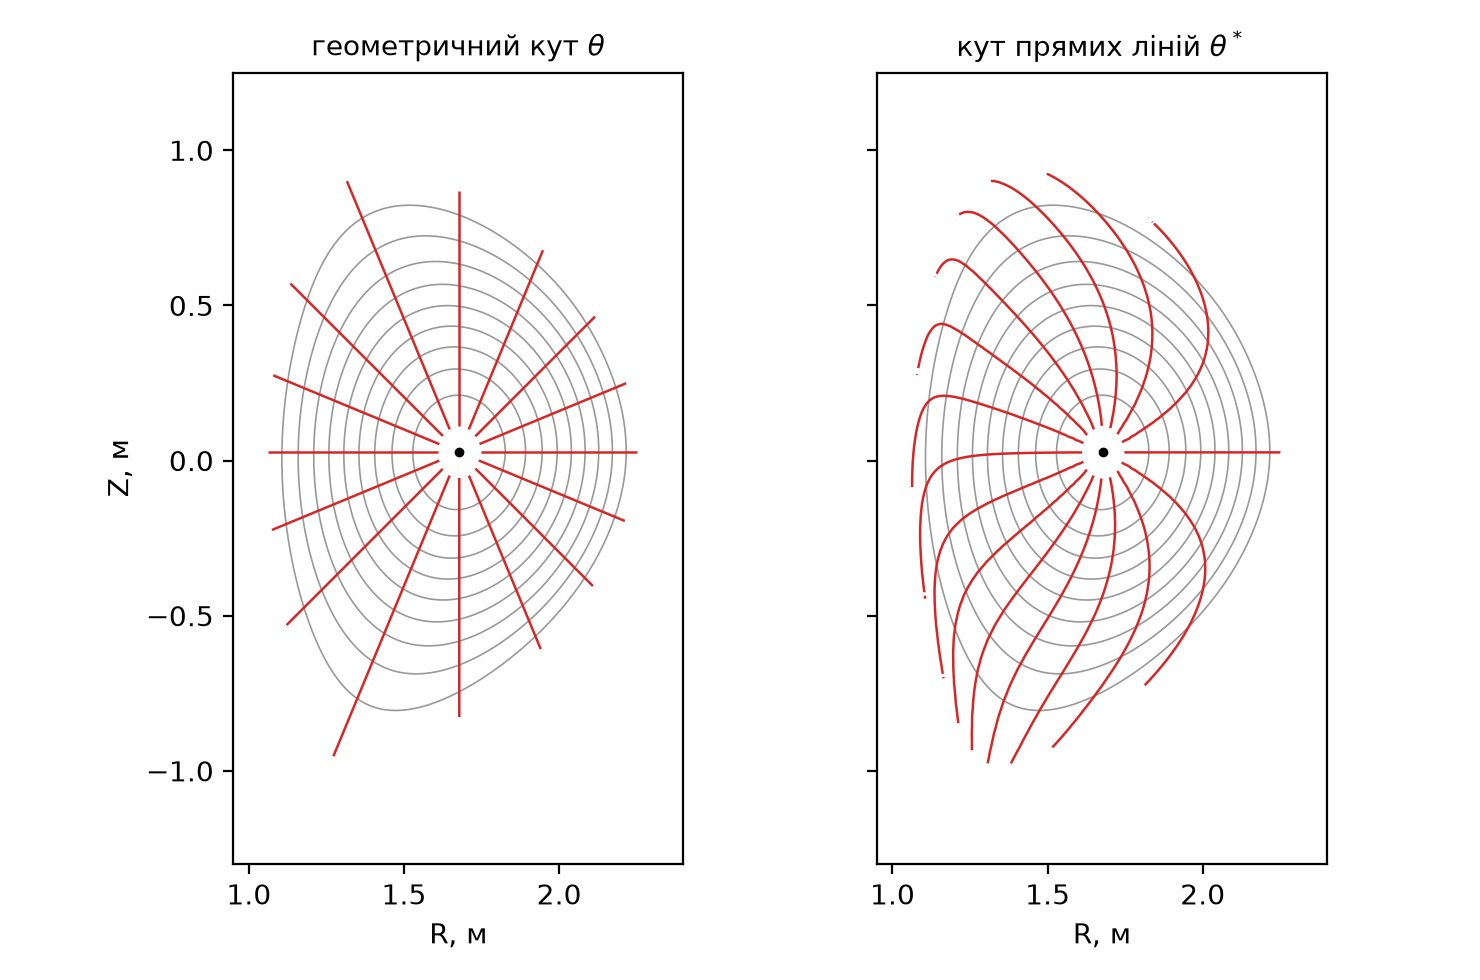
\includegraphics[width=0.86\textwidth]{geo_thetastar.jpg}
\caption{Лінії сталого кута (червоні, крок $\pi/8$) на поверхнях $\psiN=0{,}1\ldots0{,}9$ DIII-D \#203702, кадр 75. Ліворуч --- геометричний кут $\theta$ (промені з осі), праворуч --- кут прямих силових ліній $\thetastar$, відлічений від зовнішнього екватора. Лінії $\thetastar$ густі на внутрішньому боці: там силова лінія проводить більше тороїдального «часу» на одиницю полоїдальної дуги. Власний розрахунок, код: \texttt{geometry/code/geom\_tour.py}.}\label{fig:geo3-thetastar}
\end{figure}

Навіщо стільки клопоту? Збурення вигляду $\cos(m\thetastar-n\tor)$ на поверхні, де $q=m/n$, має сталу фазу вздовж силової лінії і тому \emph{резонує}: саме там виростає магнітний острів $m/n$. У геометричному куті така гармоніка «розмазується» по кількох $m$ і дає острови не там (VR1 нижче). На рис.~\ref{fig:geo3-thetastar} видно, наскільки кути різні: найбільше відхилення $|\thetastar-\theta|$ становить $15^\circ$ на $\psiN=0{,}2$, $25^\circ$ на $0{,}5$ і $48^\circ$ на $0{,}9$ (з наближенням до X-точки воно зростає).

\code{viz/src/tokviz/equilibrium.py}{363}{395}{(таблиця $\Delta=\thetastar-\theta$)}

\noindent Код табулює не сам $\thetastar$, а різницю $\Delta=\thetastar-\theta$ на регулярній сітці $(\psiN,\theta)$. Рядок 370: $\thetastar$ з накопиченої суми~\eqref{eq:geo3-thetastar}. Рядки 371--372: геометричний кут кожної точки контуру, «розгорнутий» без стрибків $2\pi$. Рядки 376--380 пропускають поверхні, де $\theta$ уздовж контуру не монотонний (біля X-точки поверхня перестає бути «зіркоподібною» відносно осі). Рядки 384--390: $\Delta$ однозначна і $2\pi$-періодична, бо обидва кути набігають рівно $2\pi$ за оберт; її інтерполюють на рівномірну сітку $\theta$. Похідні $\thetastar$ по $R$ і $Z$ далі беруть за правилом ланцюга (клас \texttt{ThetaStarField}, рядки 410--481 файлу).

\begin{established}{VE6, VR1, VR2}
Перша реалізація растеризувала $\cos(m\thetastar)$ на сітку $65\times65$. Це дало 2,4\,\% паразитної гармоніки $m=1$ і фальшивий ланцюг островів на $q=1$ ($\psiN=0{,}335$), хоча збурення містило лише $m=2$ і $3$. Аналітичне обчислення через табульовану $\Delta$ зменшило паразитну $m=1$ до 0,4\,\%, і фальшивий острів зник (VE6). Звідси два спростування: «геометричного кута достатньо для розміщення островів» (VR1) і «паразитні гармоніки з інтерполяції можна ігнорувати» (VR2)~\cite{RegViz}.
\end{established}

\begin{newfinding}[початок відліку $\thetastar$]
$\thetastar$ визначено з точністю до сталої на кожній поверхні. У \texttt{theta\_star\_geometry} ця стала --- кут першої точки контуру, яку повертає \texttt{find\_contours} (рядок 370: \texttt{cum} починається з нуля там, де почався контур). Ця точка на сусідніх поверхнях різна. Запуск \texttt{geom\_tour.py} на кадрі 75 дає: $\Delta(\theta=0)$ по 200 поверхнях таблиці лежить у межах $-79{,}7^\circ\ldots-36{,}6^\circ$, а між сусідніми поверхнями ($\delta\psiN\approx0{,}005$) стрибає до $34{,}6^\circ$.

Для $\thetastar$ на одній поверхні це неважливо, але \texttt{ThetaStarField.value\_and\_grad} бере ще й $\pa\Delta/\pa\psiN$ (рядки 479--480 файлу), і стрибки потрапляють у градієнт $\thetastar$, а через нього --- у поле збурення (\texttt{perturbation.py}, рядки 156--157). Середньоквадратичне $|\grad\thetastar|$ уздовж поверхні, рад/м:
\begin{center}\small
\begin{tabular}{@{}lccc@{}}\toprule
$\psiN$ & 0,3 & 0,6 & 0,9\\\midrule
як у коді & 38,0 & 3,9 & 3,03\\
з відліком від зовнішнього екватора & 3,5 & 2,5 & 2,89\\\bottomrule
\end{tabular}
\end{center}
На $\psiN=0{,}3$ градієнт завищено в 11 разів, на $\psiN=0{,}9$, де лежать робочі резонанси проєкту ($q=3$, $10/3$, $11/3$), --- на 5\,\%. Це узгоджується з тим, що виміряні ширини островів збігаються з формулою (VE18). \emph{Вплив на реєстр VE/VR не перевірено.} Можливе виправлення в один рядок: після рядка 390 віднімати від кожного рядка таблиці $\Delta$ його значення при $\theta=0$. Так зроблено в \texttt{geom\_tour.py}, рядки 104--109, і на рис.~\ref{fig:geo3-thetastar}.
\end{newfinding}

\section{Від перерізу до тора}\label{sec:geo3-3d}

Осесиметрія робить 3D-геометрію тривіальною: будь-який контур $(R,Z)$ --- межа плазми, поверхня $\psiN$, профіль котушки --- обертають навколо осі $Z$. Точка $(R,Z)$ на куті $\tor$ переходить у $(x,y,z)=(R\cos\tor,R\sin\tor,Z)$:

\code{viz/src/tokviz/surfaces.py}{38}{68}{(поверхня обертання)}

\noindent Рядки 52--55 --- саме ця формула для всіх точок профілю й усіх кутів одразу. Рядки 57--67 збирають чотирикутні грані між сусідніми кільцями; \texttt{\% n\_tor} і \texttt{\% n\_pol} замикають сітку по обох кутах. Параметр \texttt{scale} множить $R$ і $Z$ однаково. Для рендера проєкт збільшує DIII-D у 3 рази (\texttt{GEOMETRY\_SCALE} у \texttt{config.py}): аспектне відношення при цьому не змінюється, а отже й форма поверхонь та розташування островів у нормованих координатах.

\begin{practicum}[$q$ і $\thetastar$]
(1)~Порахуйте $q$ на $\psiN=0{,}5$ контурним інтегралом при \texttt{surface()} на сітці, згущеній удвічі (інтерполюйте $\psi$ сплайном на $129\times129$ і збудуйте нову \texttt{Equilibrium}). Наскільки зміниться $q$? (2)~Знайдіть $\psiN$ поверхні $q=1$ бісекцією по \texttt{q\_at}. (3)~Повторіть таблицю «Нового спостереження» для кадрів 10 і 150 того самого розряду. Чи змінюються стрибки початку відліку?
\end{practicum}

\chapter{Форма перерізу}\label{ch:geo4}

\section{Параметри форми}\label{sec:geo4-params}

Форму межі плазми (LCFS) описують кількома числами, які читають за її крайніми точками. Позначимо $R_{\max}$, $R_{\min}$ --- крайні радіуси, $Z_{\max}$, $Z_{\min}$ --- крайні висоти, а $R_{Z_{\max}}$, $R_{Z_{\min}}$ --- радіуси найвищої й найнижчої точок.

\begin{outofcorpus}[означення~\cite{Manual}, розд.~4]
\begin{equation}\label{eq:geo4-shape}
\begin{gathered}
R_{\mathrm{geo}}=\frac{R_{\max}+R_{\min}}2,\qquad a=\frac{R_{\max}-R_{\min}}2,\qquad A=\frac{R_{\mathrm{geo}}}a,\qquad \epsilon=\frac1A,\\
\kappa=\frac{Z_{\max}-Z_{\min}}{2a},\qquad \dup=\frac{R_{\mathrm{geo}}-R_{Z_{\max}}}a,\qquad \dlo=\frac{R_{\mathrm{geo}}-R_{Z_{\min}}}a,\qquad \delta=\frac{\dup+\dlo}2 .
\end{gathered}
\end{equation}
$A$ --- аспектне відношення, $\epsilon$ --- обернене аспектне відношення, $\kappa$ --- витягнутість (elongation), $\delta$ --- трикутність (triangularity). $\delta>0$: верхівка зсунута \emph{всередину} від $R_{\mathrm{geo}}$ (класичний D); $\delta<0$ --- назовні («перевернутий D»).
\end{outofcorpus}

У коді це кілька рядків:

\code{geo/geom_tour.py}{37}{58}{(параметри форми, площа, об'єм)}

\noindent Рядки 40--46 --- дослівно~\eqref{eq:geo4-shape}. \texttt{argmax}/\texttt{argmin} по $Z$ знаходять верхню й нижню точки. Похибка --- порядку відстані між точками контуру: для EFIT-контуру це частки сантиметра, для щільно заданої аналітичної кривої вона нехтовно мала. Рядки 53--58 --- площа перерізу за формулою Гаусса («шнурка») і об'єм тора за теоремою Паппа--Гульдіна $V=2\pi R_{\mathrm c}S$, де $R_{\mathrm c}$ --- радіус центроїда перерізу, \emph{не} $R_{\mathrm{geo}}$.

\begin{figure}[!tb]\centering
\begin{minipage}[c]{0.44\textwidth}\centering
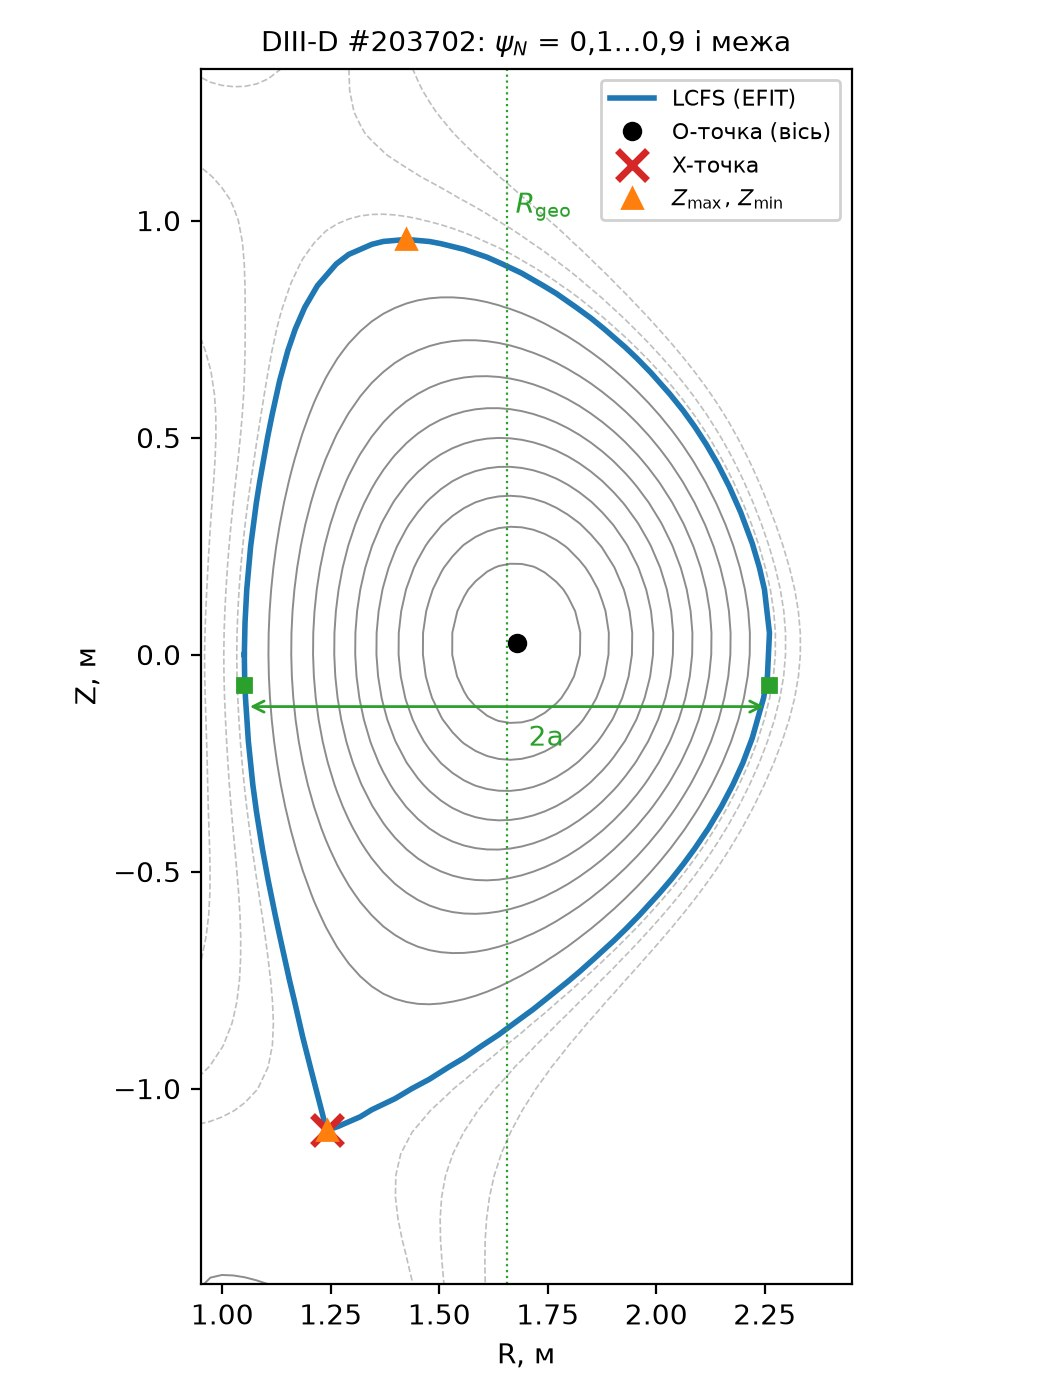
\includegraphics[width=\textwidth]{geo_diiid_shape.jpg}
\end{minipage}\hfill
\begin{minipage}[c]{0.53\textwidth}
\caption{Геометрія DIII-D \#203702, кадр 75: поверхні $\psiN=0{,}1\ldots0{,}9$ (сірі), LCFS з набору EFIT (синя), відкриті поверхні $\psiN>1$ (штрих), магнітна вісь, X-точка і точки, за якими читають параметри~\eqref{eq:geo4-shape}: крайні радіуси (квадрати), найвища й найнижча точки (трикутники). Найнижча точка межі збігається з X-точкою. Вісь зсунута від $R_{\mathrm{geo}}$ назовні (зсув Шафранова) і вгору від $Z_{\mathrm{geo}}$, бо X-точка «відтягує» низ межі. Власний розрахунок, код: \texttt{geometry/code/geom\_tour.py}; дані --- Fusion Equilibrium Challenge, CC BY 4.0.}\label{fig:geo4-diiid}
\end{minipage}
\end{figure}

\begin{table}[!tb]\centering\small
\caption{Параметри форми двох прикладів (запуск \texttt{geom\_tour.py})}\label{tab:geo4-shape}
\begin{tabular}{@{}lcc@{}}\toprule
& DIII-D \#203702, кадр 75 & JET 1975 (межа Міллера)\\\midrule
$R_{\mathrm{geo}}$, м & 1,656 & 2,960\\
$a$, м & 0,605 & 1,250\\
$A=R_{\mathrm{geo}}/a$ & 2,74 & 2,37\\
$\kappa$ & 1,70 & 1,68\\
$\dup$ / $\dlo$ & 0,38 / 0,69 & 0,348 / 0,348\\
$Z_{\mathrm{geo}}$, м & $-0{,}070$ & 0\\
площа перерізу $S$, м$^2$ & 1,77 & 8,12\\
радіус центроїда $R_{\mathrm c}$, м & 1,591 & 2,852\\
об'єм $V$, м$^3$ & 17,7 & 145,5\\
конфігурація & діверторна, нижня X-точка & лімітерна\\\bottomrule
\end{tabular}
\end{table}

Порівняння в табл.~\ref{tab:geo4-shape} повчальне: за формою перерізу DIII-D і JET дуже схожі ($A\approx2{,}4$--$2{,}7$, $\kappa\approx1{,}7$), а за розміром JET удвічі більший лінійно й у $\approx8$ разів за об'ємом. Відмінність форми --- у трикутності: DIII-D асиметричний ($\dlo\approx2\dup$), бо низ межі проходить через X-точку. JET 1975 симетричний, бо його межу задано аналітично (п.~\ref{sec:geo4-jet}).

\section{Форма Міллера}\label{sec:geo4-miller}

Щоб \emph{задати} межу кількома параметрами (а не прочитати з EFIT), найчастіше беруть параметризацію Міллера~\cite{Miller1998}:
\begin{equation}\label{eq:geo4-miller}
R(t)=R_0+a\cos\bigl(t+\arcsin\delta\,\sin t\bigr),\qquad Z(t)=\kappa a\sin t,\qquad t\in[0,2\pi).
\end{equation}
Перевірка: на $t=0$ і $\pi$ маємо $R=R_0\pm a$, тобто $R_{\mathrm{geo}}=R_0$ і півширина $a$. На $t=\pi/2$ маємо $Z=\kappa a$ і $R=R_0+a\cos(\pi/2+\arcsin\delta)=R_0-a\delta$. Отже, $\kappa$ і $\delta$ у~\eqref{eq:geo4-miller} --- \emph{точно} ті самі, що в~\eqref{eq:geo4-shape}; для JET скрипт відтворює їх до останнього знака. Повна модель Міллера містить ще радіальні похідні (зсув Шафранова $\pa R_0/\pa r$, шир витягнутості й трикутності), але для однієї межі досить~\eqref{eq:geo4-miller}.

\begin{figure}[!tb]\centering
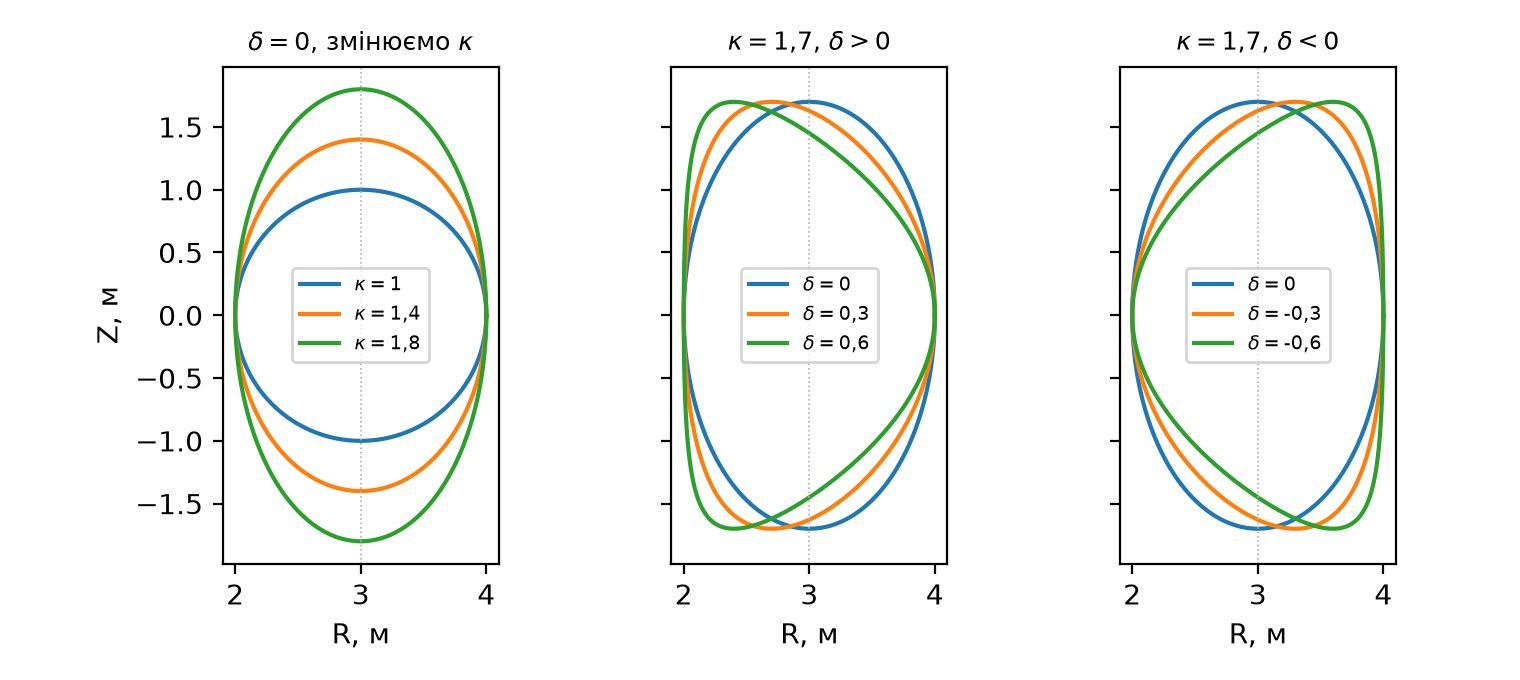
\includegraphics[width=\textwidth]{geo_miller.jpg}
\caption{Форма Міллера~\eqref{eq:geo4-miller} при $R_0=\SI{3}{м}$, $a=\SI{1}{м}$. Ліворуч: витягнутість при $\delta=0$ (еліпси). У центрі й праворуч: додатна й від'ємна трикутність при $\kappa=1{,}7$. Власний розрахунок, функція \texttt{tokviz.surfaces.d\_shape}.}\label{fig:geo4-miller}
\end{figure}

\code{viz/src/tokviz/surfaces.py}{150}{166}{(D-переріз Міллера)}

\noindent Зверніть увагу на застереження в рядках 158--160: D Міллера --- \emph{не} та «D принстонського типу», якої набуває котушка TF. Котушку визначає умова чистого натягу (п.~\ref{sec:geo6-coil}), а не параметри форми. Схожість букв --- збіг: плазмі D-форму дають котушки полоїдального поля, котушці --- магнітні сили.

\section{Навіщо плазмі форма}\label{sec:geo4-why}

\paragraph{Більший струм за того самого $q$.} Для еліптичного перерізу у циліндричному наближенні (стандартна оцінка, поза корпусом)
\begin{equation}\label{eq:geo4-qcyl}
q_{\mathrm{cyl}}\approx\frac{2\pi a^2\Bzero}{\mu_0R_0\Ip}\cdot\frac{1+\kappa^2}2 .
\end{equation}
При $\kappa=1{,}7$ множник $(1+\kappa^2)/2=1{,}95$: за тієї самої межі стійкості $q$ плазма може нести майже вдвічі більший струм, а утримання в токамаках зростає зі струмом. Проєкт JET оцінював цей виграш у $1{,}7$ раза~\cite[розд.~5]{Manual}. Точніша формула для D-перерізу з тороїдальною поправкою --- \cite[розд.~5, (5.4)]{Manual}; вона дає для JET $q(a)=5{,}99$ (розд.~\ref{ch:geo6}).

\paragraph{Ціна: вертикальна нестійкість.} Щоб витягнути плазму, потрібне зовнішнє поле з від'ємним індексом спаду; тоді плазма вертикально нестійка і потребує пасивної стінки та активного керування~\cite[розд.~4]{Manual}.

\paragraph{Трикутність і дивертор.} За стандартною теорією (поза корпусом) трикутність підвищує межі стійкості за тиском, а X-точка на кінці «трикутника» дає дивертор. Тому в DIII-D $\dlo$ більша, ніж $\dup$. Від'ємна трикутність --- окремий напрям досліджень~\cite[розд.~4]{Manual}.

\paragraph{Заповнення камери.} Кругла плазма в D-подібній камері лишає порожніми «кути». За тієї самої площі поверхні D-переріз вміщує більший об'єм; саме так аргументували форму JET~\cite[розд.~5]{Manual}.

\section{Як задали межу JET 1975}\label{sec:geo4-jet}

Проєкт JET дає $R_0=\SI{2,96}{м}$, $a=\SI{1,25}{м}$ і напіввисоту $b=\SI{2,10}{м}$ (тобто $\kappa=b/a=1{,}68$), але не дає трикутності. Натомість у ньому є таблиця 30 точок межі у верхній зовнішній чверті~\cite[с.~332]{JET1975}. Проєкт~\cite{ProjJET} підганяє до неї форму Міллера і бере з підгонки лише $\delta$:

\code{viz/src/tokviz/machine/components/plasma.py}{69}{82}{(підгонка трикутності до таблиці межі)}

\noindent Підгонка $(a_t,\kappa_t,\delta)$ методом Нелдера--Міда за середньоквадратичною відстанню від 30 точок таблиці до кривої Міллера (рядки 72--77). Крива на внутрішньому екваторі проходить через край лімітера $R=\SI{1,71}{м}$: центр \texttt{r\_in + a} (рядок 76). Рядки 79--80: два проходи з меншим кроком симплекса.

\code{viz/src/tokviz/machine/components/plasma.py}{91}{118}{(межа плазми JET)}

\noindent Рядки 99--103: з підгонки береться лише $\delta$ (округлена до $10^{-4}$), а $R_0$, $a$, $\kappa$ --- з таблиці основних параметрів проєкту. Рядки 104--113: перевірка, що плазма не перетинає стінку камери. Якщо зазор менший за допустимий, $|\delta|$ зменшують кроками. Рядки 114--115: зазори на екваторі. Результат (маніфест \texttt{data/bake\_jet1975/manifest.json}): $\delta=0{,}3476$ при середньоквадратичному відхиленні від таблиці \SI{1,7}{см}; сама підгонка дає $\kappa_t=1{,}745$, тобто таблиця витягнутіша за $b/a$. Зазори до стінки на екваторі --- \SI{17,9}{см} ззовні й \SI{4,6}{см} всередині, найменший зазор по всьому периметру --- \SI{3,5}{см}, обмеження $\delta$ не спрацювало. Сама таблиця суперечлива: її верхня точка на 9,5~см вища за $b$ і виходить за стінку, тому таблицю використано лише як \emph{форму}, а не як межу.

\begin{practicum}[форма в часі]
(1)~Для всіх кадрів DIII-D \#203702 з \texttt{efit\_lcfs\_r/z} порахуйте \texttt{shape\_params} і побудуйте $\kappa(t)$, $\dup(t)$, $\dlo(t)$. Коли з'являється X-точка (стрибок $\dlo$)? (2)~Те саме для MAST \texttt{mast\_shot\_28348}: яке аспектне відношення має сферичний токамак? (3)~Для межі Міллера JET порівняйте $S$ і $V$ з еліпсом тих самих $a$, $\kappa$ (див. задачу~\ref{pr:geo7-pappus}).
\end{practicum}

\chapter{Топологія: O-точка, X-точка, сепаратриса}\label{ch:geo5}

\section{Критичні точки і гесіан}\label{sec:geo5-crit}

Поверхні $\psi=\text{const}$ «ламаються» лише там, де $\grad\psi=0$, тобто де $\Bpol=0$. Такі точки називають критичними. Їхній тип визначає гесіан $\mathsf{H}_\psi=\bigl(\begin{smallmatrix}\psi_{RR}&\psi_{RZ}\\\psi_{RZ}&\psi_{ZZ}\end{smallmatrix}\bigr)$:
\begin{itemize}
\item $\det\mathsf{H}_\psi>0$ --- \textbf{O-точка} (еліптична): екстремум $\psi$, навколо --- вкладені замкнені контури. Це магнітна вісь або центр магнітного острова.
\item $\det\mathsf{H}_\psi<0$ --- \textbf{X-точка} (гіперболічна, сідло): крізь неї проходять дві гілки лінії рівня, що перетинаються. Ця лінія рівня --- \emph{сепаратриса}.
\end{itemize}
Докладніше (індекс Пуанкаре--Хопфа, теорія Морса) --- \cite[розд.~4, п.~4.4]{Manual}. Скрипт гайду шукає X-точку як мінімум $|\grad\psi|^2$ на сплайні і рахує $\det\mathsf{H}_\psi$ з других похідних сплайна:

\code{geo/geom_tour.py}{72}{85}{(X-точка і гесіан)}

\noindent Рядок 74: цільова функція $|\grad\psi|^2$ має мінімум нуль у \emph{будь-якій} критичній точці, тож стартова точка вирішує, яку з них знайде метод. У рядку 101 файлу старт --- найнижча точка LCFS. Рядки 81--85: $\det\mathsf{H}_\psi$ з аналітичних других похідних бікубічного сплайна. На сітці з кроком 2,7--5~см це оцінка, а не точне значення.

\section{Магнітна вісь зблизька}\label{sec:geo5-axis}

Біля O-точки $\psi-\psiax\approx\frac12\,\vect{x}^{\mathsf T}\mathsf{H}_\psi\vect{x}$, де $\vect x=(R-\Rax,Z-\Zax)$: поверхні --- подібні еліпси. Звідси два «локальні» параметри геометрії.
\begin{itemize}
\item \emph{Витягнутість на осі} $\kappa_0=\sqrt{\psi_{RR}/\psi_{ZZ}}$ (при $\psi_{RZ}\approx0$).
\item \emph{$q$ на осі.} Еліпс рівня $\delta\psi$ має площу $2\pi\,\delta\psi/\sqrt{\det\mathsf{H}_\psi}$. Тороїдальний потік через нього на радіан $\psit=(F/\Rax)\cdot\text{площа}/2\pi$, тому
\begin{equation}\label{eq:geo5-q0}
q_0=\frac{\dd\psit}{\dd\psi}=\frac{F}{\Rax\sqrt{\det\mathsf{H}_\psi}} .
\end{equation}
Цю формулу використовує \texttt{SolovevEquilibrium.q\_axis} для JET (розд.~\ref{ch:geo6}).
\end{itemize}

Для DIII-D, кадр 75: $\psi_{RR}=3{,}47$, $\psi_{ZZ}=2{,}29$, $\psi_{RZ}=-0{,}04$~Вб/(рад$\cdot$м$^2$), $\det\mathsf{H}_\psi=7{,}95>0$. Отже, $\kappa_0=1{,}23$ проти $\kappa=1{,}70$ на межі: \emph{витягнутість зростає від осі до краю}. Це типово, бо форму задають зовнішні котушки, і їхній вплив згасає вглиб плазми. За~\eqref{eq:geo5-q0} $q_0=0{,}68$, тоді як контурний інтеграл на $\psiN=0{,}02$ дає 0,711. Різниця $\approx4\,\%$ --- це межа точності других похідних сплайна на сітці $65\times65$ біля осі, а не фізика.

\section{X-точка і сепаратриса}\label{sec:geo5-x}

Для кадру 75 скрипт знаходить X-точку в $(R,Z)=(\SI{1,2407}{м},\,\SI{-1,0962}{м})$. Там $\Bpol=1{,}6\cdot10^{-9}$~Тл (чисельний нуль) і $\psiN=1{,}00002$: X-точка лежить \emph{на} LCFS і збігається з її найнижчою точкою (рис.~\ref{fig:geo4-diiid}). Це однонульова діверторна конфігурація (lower single null): межу плазми задає не стінка, а сепаратриса.

Гесіан у X-точці: $\psi_{RR}=0{,}463$, $\psi_{ZZ}=-0{,}497$, $\psi_{RZ}=-0{,}546$; власні значення $-0{,}743$ і $+0{,}710$, $\det\mathsf{H}_\psi=-0{,}53<0$ --- сідло. Звідси маленька, але гарна перевірка фізики.

\begin{derivation}[чому гілки сепаратриси перетинаються під прямим кутом]
У X-точці $\psi_R=0$, тому оператор Ґреда--Шафранова $\GSop\psi=\psi_{RR}-\psi_R/R+\psi_{ZZ}$ зводиться до сліду гесіана, а рівняння рівноваги~\cite[розд.~3]{Manual} дає $\psi_{RR}+\psi_{ZZ}=-\mu_0R_X\Jtor$, де $R_X$ --- радіус X-точки. На сепаратрисі струму майже немає, тож слід малий, і власні значення протилежні: $\lambda_1\approx-\lambda_2$. Нульова лінія квадратичної форми $\lambda_1u^2+\lambda_2v^2=0$ --- це пара прямих $v=\pm\sqrt{-\lambda_1/\lambda_2}\,u$, і при $\lambda_1=-\lambda_2$ вони перетинаються під кутом $90^\circ$. Для кадру 75 слід дорівнює $-0{,}034$ (5\,\% від $|\lambda|$), кут між гілками $\approx91^\circ$, а $|\Jtor|\approx0{,}034/(\mu_0\cdot\SI{1,24}{м})\approx\SI{2e4}{А/м^2}$. Для порівняння, середня густина струму $\Ip/S=\SI{1,36}{МА}/\SI{1,77}{м^2}\approx\SI{7,7e5}{А/м^2}$ ($|\Ip|=\SI{1,359}{МА}$ --- за законом Ампера, циркуляцією $\Bpol$ уздовж LCFS, функція \texttt{ip\_ampere} у \texttt{geom\_tour.py}, рядки 64--69), тобто в X-точці лише $\sim3\,\%$ від середньої. Точність других похідних тут та сама, що й на осі, тому число --- порядок величини.
\end{derivation}

Навколо сепаратриси простір поділено на три області:
\begin{itemize}
\item \emph{всередині LCFS} --- замкнені вкладені поверхні, «ядро» плазми;
\item \emph{SOL} (scrape-off layer) --- поверхні $\psiN>1$ над X-точкою, відкриті: силова лінія йде вздовж плазми й упирається в пластини дивертора;
\item \emph{приватна область} (private flux region) --- під X-точкою, між двома «ногами» сепаратриси. Тут також $\psiN<1$, хоча плазми ядра там немає. Тому маска «$\psiN<1$» без перевірки «всередині LCFS» захоплює цю область; на рис.~\ref{fig:geo3-thetastar} її довелося вирізати окремо.
\end{itemize}

\emph{Чому $q\to\infty$ на сепаратрисі.} У~\eqref{eq:geo3-q} підінтегральна функція $1/(R|\grad\psi|)$ біля X-точки поводиться як $1/(\text{відстань до X})$, і для поверхні, що проходить на відстані $d$ від X-точки, інтеграл росте як $\ln(1/d)$. Лінія, яка проходить поблизу X-точки, «застрягає» там на багато тороїдальних обертів. Звідси крутий ріст $q$ біля межі: $q(0{,}95)=3{,}70$, $q(0{,}98)=4{,}50$ (розд.~\ref{ch:geo3}).

\section{Як знаходять LCFS}\label{sec:geo5-lcfs}

EFIT видає LCFS разом з рівновагою, але оцінювач конкурсу Fusion Equilibrium Challenge витягає її сам із будь-якої карти $\psi$ --- і справжньої, і передбаченої. Означення: LCFS --- найнижчий рівень $\texttt{AXIS\_SIGN}\cdot\psi$, який ще дає \emph{один замкнений контур навколо осі всередині допустимої області машини}. Нижче цього рівня контур або виходить на стінку (лімітер), або розпадається в X-точці (дивертор). Рівень шукають бісекцією:

\code{fec/starter/fusion_scoring/lcfs.py}{58}{89}{(бісекція рівня LCFS)}

\noindent Рядки 68--70: вісь --- найсильніший \emph{локальний} максимум, а не глобальний (коментар у рядках 64--67: на 1,4\,\% кадрів MAST поле котушок на краю області сильніше, ніж на осі). Рядки 71--73: нижня межа бісекції --- мінімум $\phi$ на краю сітки (там контур точно відкритий), верхня --- трохи нижче осі (там точно малий замкнений контур). Рядки 80--87: 22 кроки бісекції звужують інтервал у $2^{22}\approx4\cdot10^6$ разів. \texttt{\_best\_contour\_at} (рядки 44--55) приймає контур, лише якщо він замкнений, охоплює вісь і лежить у масці камери. Цей алгоритм однаково працює для лімітерної і діверторної плазми, бо перевіряє саме топологію (замкненість і охоплення), а не тип межі.

\section{Скелет критичних точок як критерій якості}\label{sec:geo5-skeleton}

Справжня рівновага всередині LCFS має рівно одну O-точку і жодної X-точки. Шум у передбаченій $\psi$ народжує зайві пари O--X, тобто острови, яких немає. Проєкт використав це як незалежний критерій якості передбачення; повний розбір із числами (E9--E16, R5, R7, R9) є в методичці~\cite[розд.~4, п.~4.4]{Manual} і путівнику~\cite{Guide}. Тут --- лише код, що рахує індекс:

\code{ourtry/04-novelty/topology_probe.py}{63}{90}{(критичні точки через число обертів $\grad\psi$)}

\noindent Рядки 65--66: напрямок $\grad\psi$ у кожному вузлі. Рядки 69--78: для кожного вузла --- число обертів цього напрямку по 8 сусідах ($+1$ для O-точки, $-1$ для X-точки, 0 для звичайної точки); стрибки кута зводяться в $(-\pi,\pi]$ (рядок 77). Рядки 80--89: одна справжня критична точка «засвічує» блок $\approx2\times2$ вузли, тому сусідні вузли об'єднують у компоненту і рахують число обертів по периметру її обмежувального прямокутника. Так кожну точку враховано один раз.

\begin{established}{E9--E11}
На кадрах DIII-D \#203702 без шуму скелет --- 1 O-точка, 0 X-точок, сума індексів $+1$. Скелет стійкий до шуму 3\,\% від $\mathrm{std}(\psi)$. При 10\,\% з'являється $\approx20$ зайвих точок, але сума індексів лишається $\approx+1$, бо точки народжуються парами O--X. Тому інформативна \emph{кількість} точок, а не їхня сума~\cite{RegEst}, \cite[розд.~4]{Manual}.
\end{established}

\begin{practicum}[топологія]
(1)~Запустіть \texttt{find\_x\_point} зі старту на вісі. Що знайде метод і чому? (2)~Знайдіть другу (верхню) критичну точку DIII-D поза LCFS, стартувавши над верхньою точкою межі. Яке в неї $\psiN$ і $\det\mathsf{H}_\psi$? Наскільки розряд далекий від double null? (3)~У \texttt{topology\_probe.py} вимкніть ерозію (\texttt{erode=0}) і поясніть, чому сума індексів стає $1-k_X$.
\end{practicum}

\chapter{Геометрія JET: від плазми до котушок}\label{ch:geo6}

Попередні розділи йшли від $\psi$ до форми. Тут --- навпаки: від вимог до форми машини. Приклад --- проєкт JET 1975~р.~\cite{JET1975}, за яким проєкт має 3D-реконструкцію~\cite{ProjJET}. Повна «анатомія» з механікою, камерою, трансформатором і портами --- у методичці~\cite[розд.~5]{Manual}. Тут лише те, що стосується геометрії, і код, що її рахує.

\section{Аспектне відношення як компроміс}\label{sec:geo6-aspect}

Струм котушок TF, потрібний для заданих $\Ip$ і $q$, зростає як $(R_0/a)^2$~\cite[розд.~5, (5.1)]{Manual}, тому магніт дешевшає зі зменшенням $A$. Знизу $A$ обмежує центральний стовп: крізь отвір тора треба провести внутрішні ноги котушок TF і осердя трансформатора, яке наводить струм. Проєкт знайшов мінімум $A\approx2{,}2$ і обрав $R_0/a=2{,}37$~\cite[розд.~5]{Manual}. Табл.~\ref{tab:geo4-shape} показує той самий порядок у DIII-D ($A=2{,}74$). Ціна малого $A$ --- більше захоплених частинок: для зовнішньої поверхні JET $\sqrt{2\epsilon/(1+\epsilon)}=0{,}77$ при $\epsilon=a/R_0=0{,}42$~\cite[розд.~5]{Manual}.

\begin{figure}[!tb]\centering
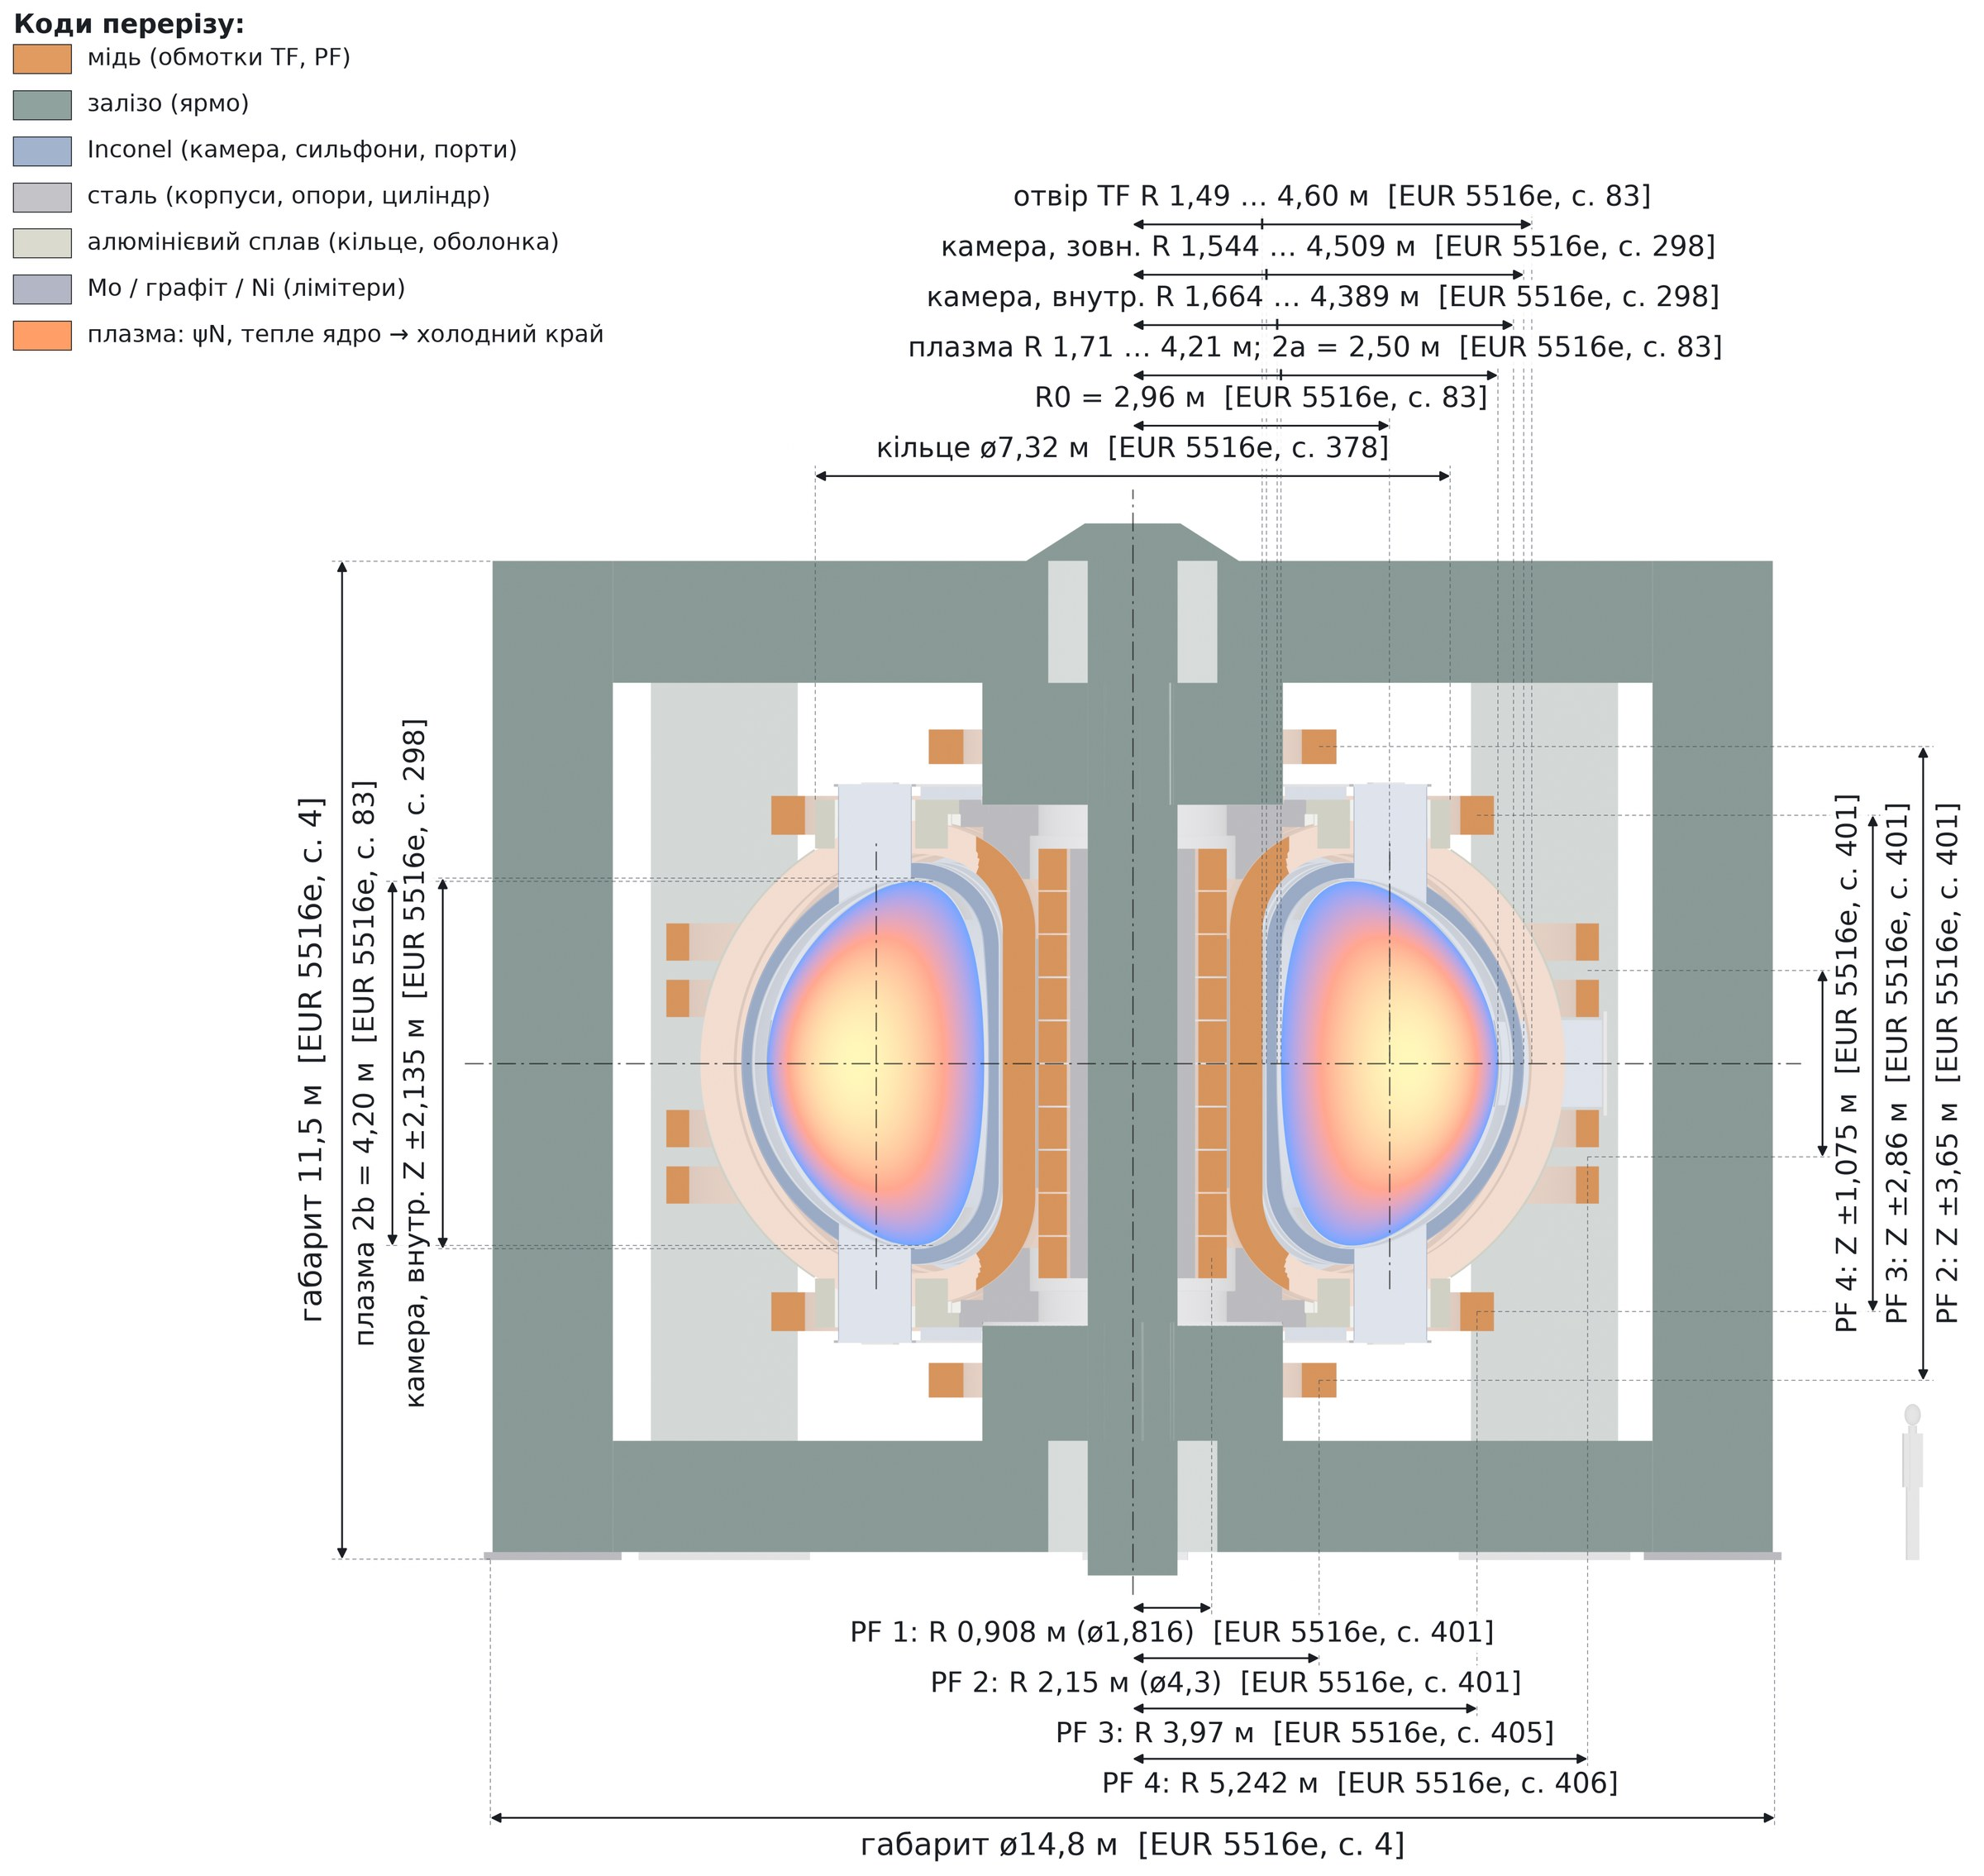
\includegraphics[width=0.84\textwidth]{jet_section.jpg}
\caption{Вертикальний переріз JET 1975 з розмірами: від осі назовні --- центральна колона ярма, стек PF-1, внутрішня нога TF, камера, плазма ($\psiN$), зовнішня нога TF, PF-2--4, вертикальні плечі. Власна 3D-реконструкція~\cite{ProjJET} (рисунок з методички~\cite[розд.~5]{Manual}); побудовано за даними~\cite{JET1975}.}\label{fig:geo6-section}
\end{figure}

\section{Котушка TF: D чистого натягу}\label{sec:geo6-coil}

Котушка TF розтягується магнітним тиском назовні. Кругла котушка при цьому згинається, а згин руйнує ізоляцію між витками. D-подібна котушка сприймає навантаження \emph{лише натягом}, без згину. Умова цього --- радіус кривини контуру, пропорційний $R$~\cite[розд.~5, (5.3)]{Manual}:
\begin{equation}\label{eq:geo6-D}
\rho(R)=\kD R,\qquad \kD=\tfrac12\ln\frac{R_2}{R_1},
\end{equation}
де $R_1$ --- верх прямої внутрішньої ноги, $R_2$ --- зовнішній екватор. Для осьової лінії обмотки нашої моделі $R_1=\SI{1,304}{м}$, $R_2=\SI{4,790}{м}$~\cite[розд.~5]{Manual}, звідки $\kD=0{,}651$: радіус кривини $\SI{0,85}{м}$ біля внутрішньої ноги і $\SI{3,12}{м}$ на зовнішньому екваторі. Контур круто загинається всередині і полого --- зовні; разом із прямою ногою це й дає літеру D. Як уже сказано в п.~\ref{sec:geo4-miller}, це \emph{інша} крива, ніж D Міллера для плазми (див. також VR6: проєкт свідомо не наводить замкненої формули кривої Princeton D~\cite{RegViz}). У коді котушку не будують з~\eqref{eq:geo6-D}: контур отвору оцифровано з креслення проєкту (\texttt{machines/jet1975/profiles/tf\_coil\_inner.csv}) і зсунуто на половину товщини ноги.

\section{Гофрування тороїдального поля}\label{sec:geo6-ripple}

32 окремі котушки порушують осесиметрію: $|\Bvec|$ стає періодичним по $\tor$ з періодом $2\pi/32$. Глибину гофрування рахують так: $\dripple=(B_{\max}-B_{\min})/(B_{\max}+B_{\min})$, де $B_{\max}$ --- у площині котушки, $B_{\min}$ --- посередині між котушками. \emph{Пастка:} проєкт JET означує $\eripple=2\dripple$~\cite[розд.~5]{Manual}. Код рахує обидва варіанти за законом Біо--Савара від 32 ниток уздовж осьової лінії обмотки:

\code{viz/src/tokviz/machine/ripple.py}{122}{137}{(гофрування за Біо--Саваром)}

\noindent Рядки 131--133: $|\Bvec|$ у площині котушки ($\tor_0$) і посередині між котушками ($\tor_0+\pi/32$) у тих самих точках $(R,Z)$. Рядки 135--137: обидва означення. Відношення не залежить від струму, бо поле лінійне за ним.

\begin{projmodel}[гофрування JET]
Запуск \texttt{geom\_tour.py} (41~МА, одна нитка на котушку): на краю плазми $R=\SI{4,21}{м}$ $\dripple=1{,}83\,\%$, тобто $\eripple=3{,}67\,\%$ проти проєктних 3,6\,\%; на осі $R_0$ $\dripple=3\cdot10^{-7}$; $B(R_0)=\SI{2,770}{Тл}$, як у проєкті (2,77). Похибку дає переважно оцифрування контуру котушки: зсув осьової лінії на $\pm\SI{2}{см}$ змінює $\eripple(\SI{4,21}{м})$ на $+14/-12\,\%$~\cite[розд.~5]{Manual}.
\end{projmodel}

Чому гофрування так круто зростає назовні? Грубо (поза корпусом): поле дискретних ниток з кроком $2\pi R_2/N$ на радіусі $R_2$ спадає всередину як $(R/R_2)^N$. Для $N=32$ оцінка $(4{,}21/4{,}79)^{32}=1{,}6\,\%$ близька до 1,83\,\% за Біо--Саваром. Плазма JET займає отвір майже до зовнішньої ноги, і за це доводиться платити гофруванням.

\section{Рівновага в межі JET}\label{sec:geo6-solovev}

Щоб побачити магнітні поверхні всередині D-межі (п.~\ref{sec:geo4-jet}), потрібна рівновага. Найпростіша точна --- рівновага Соловйова: при сталих $\mu_0p'$ і $FF'$ рівняння Ґреда--Шафранова лінійне. Його розв'язок --- частинний поліном плюс сім однорідних розв'язків~\cite{Cerfon2010}. Сім коефіцієнтів задають так, щоб межа $\psi=0$ проходила через три точки D (зовнішній і внутрішній екватор, верх) з правильним нахилом і кривинами Міллера:

\code{viz/src/tokviz/machine/equilibrium_analytic.py}{283}{303}{(сім умов Cerfon--Freidberg)}

\noindent Рядки 283--285: $\epsilon=a/R_0$, $\arcsin\delta$ і частинний розв'язок $u_p$ ($A$ --- параметр поділу струму між тиском і $FF'$). Рядки 288--290: кривини межі Міллера на зовнішньому екваторі, внутрішньому екваторі й у верхній точці. Рядок 291: ці три точки в безрозмірних координатах $x=R/R_0$, $y=Z/R_0$. Рядки 296--300: сім умов --- $u=0$ у трьох точках, $\pa u/\pa x=0$ у верхній точці (там дотична горизонтальна) і три умови кривини. Рядок 303: лінійна система $7\times7$.

Лишаються два вільні параметри. Параметр $A$ підбирають бісекцією так, щоб $\betap=0{,}9$ (як у виносках проєкту), а масштаб $\psi_0$ --- так, щоб $\Ip=\SI{3,8}{МА}$:

\code{viz/src/tokviz/machine/equilibrium_analytic.py}{490}{517}{(збирання рівноваги JET)}

\noindent Рядки 501--506: $\kappa=b/a$, бісекція по $A$ для заданої $\betap$, розв'язок форми і масштаб $\psi_0$ під $\Ip$. Рядки 507--509: $\psi$ розраховують на сітці $193\times257$ із запасом за межею плазми і загортають у той самий клас \texttt{Equilibrium}, що й кадри EFIT. Тому весь код розд.~\ref{ch:geo2}--\ref{ch:geo5} (поверхні, $q$, $\thetastar$) працює для JET без змін.

\begin{table}[!tb]\centering\small
\caption{Рівновага Соловйова в межі JET 1975 (запуск \texttt{geom\_tour.py}; ті самі числа --- у \texttt{data/bake\_jet1975/physics.json}~\cite{ProjJET})}\label{tab:geo6-eq}
\begin{tabular}{@{}ll@{\hspace{2.5em}}ll@{}}\toprule
$A$ (поділ струму) & 0,0948 & $\Ip$ & 3,80~МА \\
$\psi_0$ & 15,64~Вб/рад & $\betap$ / $\betat$ & 0,900 / 2,32\,\% \\
нев'язка межі & 0,08~мм & $\li(1)$ / $\li(3)$ & 0,498 / 0,425 \\
вісь $\Rax$ & 3,183~м & зсув Шафранова $\Rax-R_0$ & 0,223~м \\
$q_0$ (з гесіана) & 2,80 & $\qnf$ / $q(0{,}99)$ & 5,51 / 5,75 \\
об'єм (квадратура) & 145,46~м$^3$ & об'єм (Папп, табл.~\ref{tab:geo4-shape}) & 145,46~м$^3$ \\\bottomrule
\end{tabular}
\end{table}

\begin{figure}[!tb]\centering
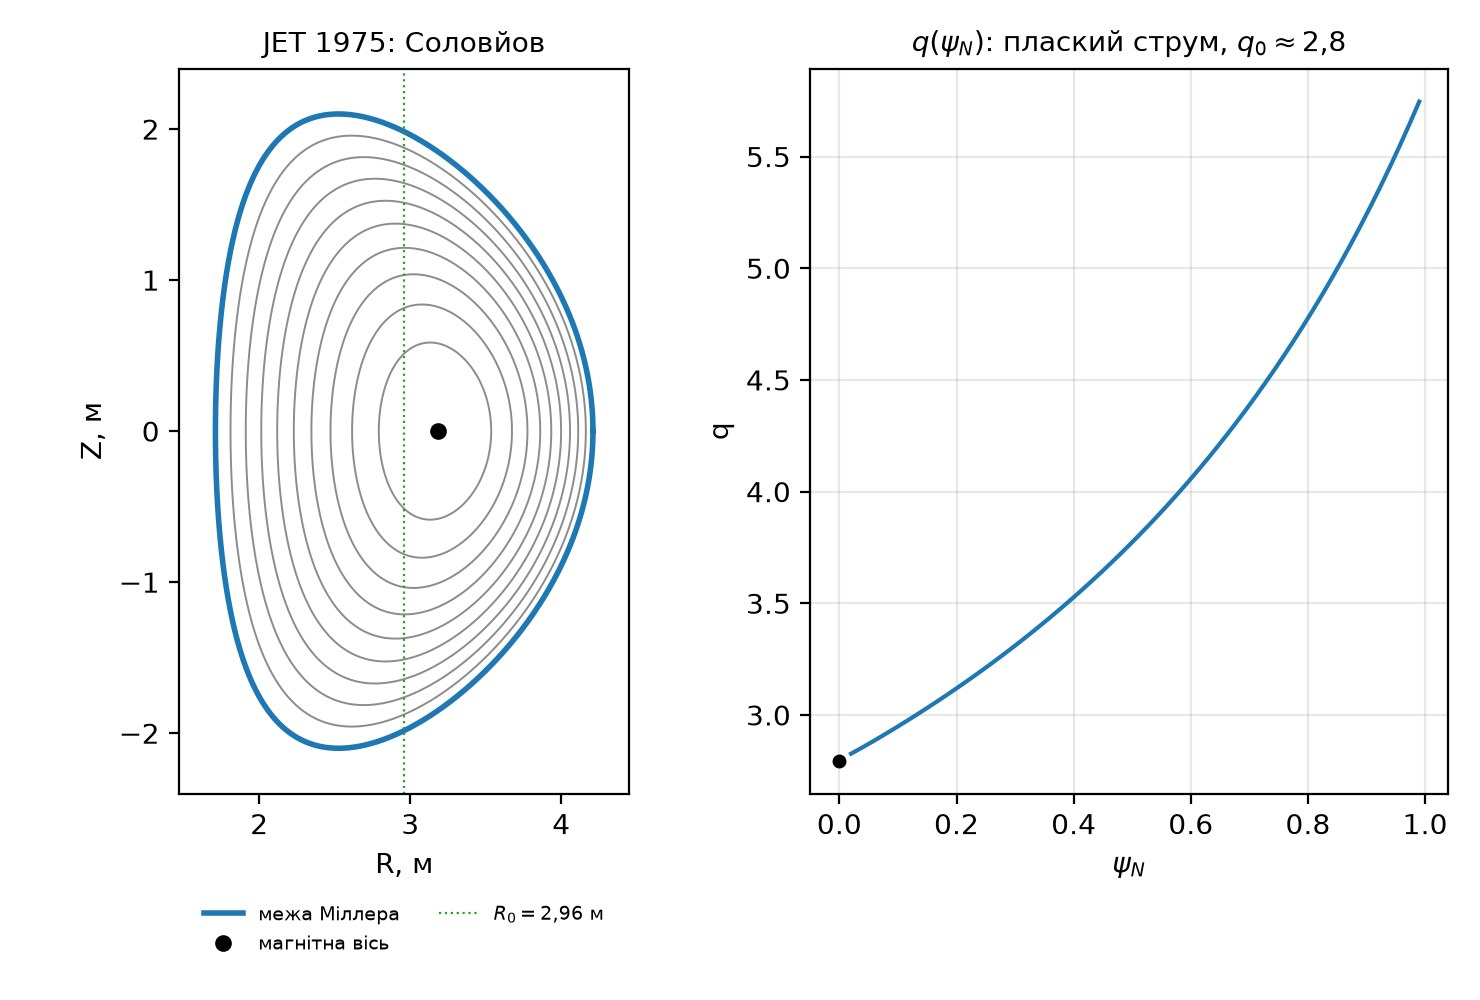
\includegraphics[width=0.86\textwidth]{geo_jet_solovev.jpg}
\caption{Рівновага Соловйова в межі JET 1975. Ліворуч: поверхні $\psiN=0{,}1\ldots0{,}9$, межа Міллера ($\kappa=1{,}68$, $\delta=0{,}348$) і магнітна вісь, зсунута на \SI{0,22}{м} назовні від $R_0$. Праворуч: $q(\psiN)$ з контурного інтеграла~\eqref{eq:geo3-q} і $q_0$ з гесіана~\eqref{eq:geo5-q0} (точка). Власний розрахунок, код: \texttt{geometry/code/geom\_tour.py}.}\label{fig:geo6-solovev}
\end{figure}

Об'єм, обчислений квадратурою по сітці, збігається з об'ємом за Паппом (п.~\ref{sec:geo4-params}) з відносною різницею $10^{-5}$ --- незалежна перевірка обох кодів. Контурний $q$ і $q$ з трасування силових ліній збігаються до 0,015\,\% на $\psiN=0{,}1\ldots0{,}95$ (\texttt{physics.json}, ключ \texttt{q\_traced\_vs\_contour}). Помітний і зсув Шафранова: вісь на \SI{0,22}{м} зовні від $R_0$ (рис.~\ref{fig:geo6-solovev}), а поверхні згущуються до зовнішнього боку.

\emph{Чесне обмеження.} Струм Соловйова пласкої форми: $\Jtor=(C_1R+C_2/R)/\mu_0$ від $\psi$ не залежить. Тому $q_0=2{,}80$ і $q(a)/q_0\approx2{,}1$, тоді як проєкт розраховував на пікований струм з $q_0\approx1$. Поверхонь $q=1$, $3/2$, $2$ у цій моделі немає. Для топології (вкладені поверхні, замикання раціональних ліній $q=3,\,7/2,\,4,\,5$ з точністю $<\SI{0,5}{мм}$) модель придатна, для МГД-стійкості --- ні~\cite[розд.~5]{Manual}.

\begin{practicum}[JET]
(1)~Побудуйте рівновагу з \texttt{method="lsq"} замість \texttt{"cf7"}: як зміняться нев'язка межі і $q_0$? (2)~Змініть $\delta$ на 0 і на 0,5 (\texttt{build\_equilibrium(delta=...)}): як залежать $\qnf$ і зсув Шафранова від трикутності? (3)~Порахуйте $\dripple$ на $R=4{,}0\ldots4{,}4$~м з кроком 5~см і порівняйте з оцінкою $(R/R_2)^{32}$. Де оцінка найгірша і чому?
\end{practicum}

\chapter{Практикум і задачі}\label{ch:geo7}

\section{Контрольні запитання}\label{sec:geo7-q}

\begin{enumerate}
\item Чому вся геометрія осесиметричної рівноваги задається однією функцією $\psi(R,Z)$? Що саме порушує осесиметрію в реальній машині?
\item Чому в таблицях і графіках поверхні позначають через $\psiN$, а не через $\psi$? Що станеться з $\psiN$, якщо помножити $\psi$ на $-1$?
\item Чому $\qnf$, а не $q$ на межі? Що відбувається з $q$ на сепаратрисі?
\item Чим кут $\thetastar$ кращий за геометричний $\theta$ для опису островів? Чому лінії сталого $\thetastar$ густіші на внутрішньому боці тора?
\item Чому $\thetastar$ не залежить від $F$, а $q$ залежить лінійно?
\item Чим відрізняються D Міллера (плазма) і D чистого натягу (котушка TF)? Що визначає кожну з них?
\item Чому гілки сепаратриси перетинаються майже під прямим кутом? Коли кут відрізнявся б від $90^\circ$?
\item Чому маска «$\psiN<1$» не збігається з областю «всередині LCFS» у діверторній плазмі?
\end{enumerate}

\section{Задачі}\label{sec:geo7-p}

\begin{enumerate}
\item\label{pr:geo7-miller} \emph{Міллер.} Доведіть, що в параметризації~\eqref{eq:geo4-miller} верхня точка має $R=R_0-a\delta$ і $Z=\kappa a$, тобто $\kappa$ і $\delta$ збігаються з означеннями~\eqref{eq:geo4-shape}. Обчисліть $R_{Z_{\max}}$ для JET ($R_0=\SI{2,96}{м}$, $a=\SI{1,25}{м}$, $\delta=0{,}3476$).
\item\label{pr:geo7-qcyl} \emph{Виграш від витягнутості.} За~\eqref{eq:geo4-qcyl} оцініть $q_{\mathrm{cyl}}$ для DIII-D \#203702 ($a=\SI{0,605}{м}$, $\kappa=1{,}70$, $R_{\mathrm{geo}}=\SI{1,656}{м}$, $\Btor(R_{\mathrm{geo}})=\SI{1,953}{Тл}$, $|\Ip|=\SI{1,359}{МА}$) з урахуванням і без урахування $\kappa$. Порівняйте з $\qnf=3{,}70$. Що може пояснити різницю?
\item\label{pr:geo7-pappus} \emph{Площа й об'єм.} Для JET порівняйте площу й об'єм межі Міллера (табл.~\ref{tab:geo4-shape}) з еліпсом тих самих $a$, $\kappa$ з центром на $R_0$. Чому трикутність зменшує об'єм помітніше, ніж площу?
\item\label{pr:geo7-axis} \emph{Вісь.} За гесіаном на осі DIII-D ($\psi_{RR}=3{,}473$, $\psi_{ZZ}=2{,}288$, $\psi_{RZ}=-0{,}036$~Вб/(рад$\cdot$м$^2$)), $F=\SI{3,2334}{Т.м}$ і $\Rax=\SI{1,6782}{м}$ знайдіть $\kappa_0$ і $q_0$ за~\eqref{eq:geo5-q0}. Виведіть~\eqref{eq:geo5-q0}.
\item\label{pr:geo7-x} \emph{X-точка.} Власні значення гесіана в X-точці DIII-D --- $-0{,}743$ і $+0{,}710$~Вб/(рад$\cdot$м$^2$), $R_X=\SI{1,241}{м}$. Знайдіть кут між гілками сепаратриси і густину струму $|\Jtor|$ в X-точці. Порівняйте з середньою $|\Ip|/S$.
\item\label{pr:geo7-coil} \emph{D-котушка.} Для $R_1=\SI{1,304}{м}$, $R_2=\SI{4,790}{м}$ знайдіть $\kD$ і радіуси кривини на кінцях дуги. Наскільки менший радіус біля внутрішньої ноги, ніж на зовнішньому екваторі?
\item\label{pr:geo7-ripple} \emph{Гофрування.} Оцініть $\dripple$ на $R=\SI{4,21}{м}$ і на $R_0=\SI{2,96}{м}$ як $(R/R_2)^N$ при $N=32$. Порівняйте з Біо--Саваром ($1{,}83\,\%$ і $3\cdot10^{-7}$). Чому на осі проста оцінка непридатна?
\end{enumerate}

\begin{practicum}[міні-проєкт]
Напишіть функцію, яка для будь-якого кадру DIII-D чи MAST за 1~с повертає «паспорт геометрії»: $\Rax$, $\Zax$, $R_{\mathrm{geo}}$, $a$, $A$, $\kappa$, $\dup$, $\dlo$, $S$, $V$, $|\Ip|$, координати й $\psiN$ X-точок, $q_0$ (з гесіана), $\qnf$. Усі цеглинки вже є в \texttt{geom\_tour.py} і \texttt{tokviz.equilibrium}. Перевірте на кадрі 75: паспорт має відтворити числа розд.~\ref{ch:geo2}--\ref{ch:geo5}.
\end{practicum}

\appendix
\chapter{Відповіді і шпаргалка}\label{ch:geoA}

\section{Відповіді до задач}\label{sec:geoA-ans}

\begin{enumerate}
\item На $t=\pi/2$: $\sin t=1$, $Z=\kappa a$ --- максимум $Z$, отже $\kappa=Z_{\max}/a$; $R=R_0+a\cos(\pi/2+\arcsin\delta)=R_0-a\sin(\arcsin\delta)=R_0-a\delta$, отже $(R_{\mathrm{geo}}-R_{Z_{\max}})/a=\delta$. JET: $R_{Z_{\max}}=2{,}96-1{,}25\cdot0{,}3476=\SI{2,5255}{м}$ (збігається з \texttt{geom\_tour.json}).
\item З $\kappa$: $q_{\mathrm{cyl}}=3{,}08$; без $\kappa$: 1,59. Реальне $\qnf=3{,}70$ ще на 20\,\% більше: формула~\eqref{eq:geo4-qcyl} не враховує тороїдальності ($\epsilon=0{,}37$), трикутності й того, що $\qnf$ береться поблизу X-точки, де $q$ круто зростає (п.~\ref{sec:geo5-x}).
\item Еліпс: $S=\pi a^2\kappa=\SI{8,25}{м^2}$, $V=2\pi R_0S=\SI{153,4}{м^3}$. Міллер: $S=\SI{8,12}{м^2}$ ($-1{,}6\,\%$), $V=\SI{145,5}{м^3}$ ($-5{,}2\,\%$). Трикутність переносить верх і низ перерізу всередину: центроїд зсувається з $R_0=\SI{2,96}{м}$ на $R_{\mathrm c}=\SI{2,852}{м}$, а $V=2\pi R_{\mathrm c}S$ чутливий до $R_{\mathrm c}$.
\item $\kappa_0=\sqrt{3{,}473/2{,}288}=1{,}23$. $\det\mathsf{H}_\psi=3{,}473\cdot2{,}288-0{,}036^2=7{,}95$; $q_0=3{,}2334/(1{,}6782\cdot\sqrt{7{,}95})=0{,}68$. Виведення: еліпс $\frac12\vect x^{\mathsf T}\mathsf{H}\vect x=\delta\psi$ має площу $2\pi\delta\psi/\sqrt{\det\mathsf H}$; тороїдальний потік на радіан $\psit=\Btor\cdot\text{площа}/2\pi=F\,\delta\psi/(\Rax\sqrt{\det\mathsf H})$; $q=\dd\psit/\dd\psi$.
\item Нульова лінія $\lambda_1u^2+\lambda_2v^2=0$: $v/u=\pm\sqrt{0{,}743/0{,}710}=\pm1{,}023$, кут кожної гілки до осі $u$ --- $45{,}7^\circ$, між гілками --- $91{,}3^\circ$. $|\Jtor|=|\lambda_1+\lambda_2|/(\mu_0R_X)=0{,}033/(1{,}257\cdot10^{-6}\cdot1{,}241)\approx\SI{2,1e4}{А/м^2}$; $|\Ip|/S=1{,}359\cdot10^6/1{,}769=\SI{7,7e5}{А/м^2}$, відношення $\approx3\,\%$.
\item $\kD=\frac12\ln(4{,}790/1{,}304)=0{,}651$; $\rho(R_1)=\SI{0,85}{м}$, $\rho(R_2)=\SI{3,12}{м}$ --- у $R_2/R_1=3{,}67$ раза менший.
\item $(4{,}21/4{,}79)^{32}=1{,}6\,\%$ проти 1,83\,\% --- непогано. На осі $(2{,}96/4{,}79)^{32}=2\cdot10^{-7}$ --- порядок збігається випадково: на осі вже важать внески внутрішніх ніг ($\propto(R_1/R)^{32}$) і скінченна довжина контуру, яких оцінка не містить.
\end{enumerate}

\paragraph{Практикуми.} Розд.~\ref{ch:geo5}, п.~(1): зі старту біля осі метод знаходить саму вісь (1,67817; 0,02623)~м --- у ній теж $|\grad\psi|=0$. П.~(2): верхня критична точка лежить у $(\SI{1,170}{м},\,\SI{1,149}{м})$, $\psiN=1{,}058$, $\det\mathsf{H}_\psi=-0{,}32$ --- сідло поза LCFS. Розряд однонульовий, але друга X-точка лише на $\Delta\psiN\approx0{,}06$ «зовні». Інші практикуми відкриті; числа --- з вашого запуску.

\section{Шпаргалка}\label{sec:geoA-cheat}

\begin{cheat}[формули гайду]
\small
\begin{tabular}{@{}p{0.33\textwidth}p{0.62\textwidth}@{}}
Поле & $\Bvec=\grad\psi\times\grad\tor+F\grad\tor$; $\BR=-\psi_Z/R$, $\BZ=\psi_R/R$, $\Btor=F/R$, $\Bpol=|\grad\psi|/R$\\[2pt]
Нормований потік & $\psiN=(\psi-\psiax)/(\psib-\psiax)$\\[2pt]
Запас стійкості & $q=\frac{F}{2\pi}\oint\frac{\dd\ell}{R|\grad\psi|}$, \quad $q_0=\frac{F}{\Rax\sqrt{\det\mathsf{H}_\psi}}$\\[2pt]
Кут прямих ліній & $\thetastar=2\pi\int_0^\ell\frac{\dd\ell'}{R|\grad\psi|}\Big/\oint\frac{\dd\ell'}{R|\grad\psi|}$, \quad $\dd\thetastar/\dd\tor=1/q$\\[2pt]
Форма & $R_{\mathrm{geo}}=\frac{R_{\max}+R_{\min}}2$, $a=\frac{R_{\max}-R_{\min}}2$, $\kappa=\frac{Z_{\max}-Z_{\min}}{2a}$, $\delta_{\mathrm{u,l}}=\frac{R_{\mathrm{geo}}-R_{Z_{\max,\min}}}a$\\[2pt]
Міллер & $R=R_0+a\cos(t+\arcsin\delta\sin t)$, $Z=\kappa a\sin t$\\[2pt]
Площа, об'єм & $S=\frac12\sum(R_iZ_{i+1}-R_{i+1}Z_i)$, \quad $V=2\pi R_{\mathrm c}S$\\[2pt]
Струм плазми & $\Ip=\mu_0^{-1}\oint\Bpol\cdot\dd\vect{\ell}$ по LCFS\\[2pt]
Критичні точки & $\grad\psi=0$; $\det\mathsf{H}_\psi>0$ --- O, $<0$ --- X; у X-точці $\psi_{RR}+\psi_{ZZ}=-\mu_0R\Jtor$\\[2pt]
D-котушка & $\rho=\kD R$, $\kD=\frac12\ln(R_2/R_1)$\\[2pt]
Гофрування & $\dripple=\frac{B_{\max}-B_{\min}}{B_{\max}+B_{\min}}$, JET 1975: $\eripple=2\dripple$\\
\end{tabular}
\end{cheat}

\begin{cheat}[числа прикладів]
\small
\begin{tabular}{@{}lll@{}}
& DIII-D \#203702, кадр 75 & JET 1975 (модель)\\\midrule
вісь $(\Rax,\Zax)$, м & (1,678; 0,026) & (3,183; 0)\\
$R_{\mathrm{geo}}$, $a$, $A$ & 1,656~м; 0,605~м; 2,74 & 2,96~м; 1,25~м; 2,37\\
$\kappa$; $\dup/\dlo$ & 1,70; 0,38/0,69 & 1,68; 0,348/0,348\\
$S$, $V$ & 1,77~м$^2$; 17,7~м$^3$ & 8,12~м$^2$; 145,5~м$^3$\\
$|\Ip|$; $\Btor$ на осі & 1,36~МА; 1,93~Тл & 3,80~МА; 2,77~Тл (вакуум, $R_0$)\\
$q_0$; $\qnf$ & 0,68--0,71; 3,70 & 2,80; 5,51\\
X-точка & (1,241; $-1{,}096$)~м, $\psiN=1$ & немає (лімітер)\\
\end{tabular}
\end{cheat}

% Бібліографія гайду по геометрії. Записи проєкту взято з manual/bib/bibliography.tex і guide/bib/refs_project.tex.
\begin{thebibliography}{99}
\footnotesize\raggedright
\addcontentsline{toc}{chapter}{Бібліографія}

\bibitem{Manual} Фізика плазми всередині токамака~: навчальний посібник (методичка)~/ \texttt{manual/main.pdf}. -- 2026.
  Розд.~3 (рівновага), 4 (геометричні ефекти), 5 (анатомія токамака: JET).

\bibitem{Guide} Путівник гіпотезами проєкту~/ \texttt{guide/main.pdf}. -- 2026.

\bibitem{RegEst} Реєстр встановленого (E1--E35, R1--R9)~/ \texttt{Our try/00-decisions/ESTABLISHED.md}. -- Ред. 2026-09-29.

\bibitem{RegViz} Реєстр візуалізації (VE, VR, VC, VQ)~/ \texttt{tokamak-3d-viz/findings.md}. -- Ред. 2026-09-29.

\bibitem{ProjViz} tokamak-3d-viz~: візуалізація рівноваги DIII-D \#203702 (кадр 75, $t=1760$~мс),
  трасування силових ліній, острови, перерізи Пуанкаре~: програмний код (MIT)~/
  тека \texttt{tokamak-3d-viz}; опис конвенцій --- \texttt{docs/PHYSICS.md}. -- 2026. Дані рівноваги: Fusion Equilibrium Challenge
  (Sophelio / General Atomics), CC BY 4.0.

\bibitem{ProjJET} tokamak-3d-viz~: 3D-реконструкція JET (проєкт 1975 і стан 1983) --- база розмірів
  \texttt{machines/jet1975}, геометричне ядро, рівновага Соловйова, гофрування~: програмний код~/
  тека \texttt{tokamak-3d-viz}; опис --- \texttt{docs/JET-EQUILIBRIUM.md}. -- 2026.

\bibitem{FEC2026} Nakkina et al. The Fusion Equilibrium Challenge: Inferring Magnetic Geometry
  Without Magnetic Diagnostics~// arXiv:2609.01750. -- 2026. Набір даних
  \texttt{Sophelio/fusion-equilibrium-challenge}, CC BY 4.0.

\bibitem{JET1975} The JET Project~: Design Proposal for the Joint European Torus~: EUR 5516e (EUR-JET-R5). --
  Luxembourg~: Commission of the European Communities, 1976. -- 678~p. -- © CECA, CEE, CEEA.

\bibitem{Cerfon2010} Cerfon~A.\,J., Freidberg~J.\,P. «One size fits all» analytic solutions to the Grad--Shafranov
  equation~// Physics of Plasmas. -- 2010. -- Vol.~17, No.~3. -- 032502. -- DOI: 10.1063/1.3328818.
  (Поза корпусом; використано лише як метод у коді проєкту.)

\bibitem{Miller1998} Miller~R.\,L., Chu~M.\,S., Greene~J.\,M., Lin-Liu~Y.\,R., Waltz~R.\,E. Noncircular, finite aspect
  ratio, local equilibrium model~// Physics of Plasmas. -- 1998. -- Vol.~5, No.~4. -- P.~973--978.
  (Поза корпусом; джерело параметризації D-перерізу.)

\end{thebibliography}

\end{document}
